\documentclass[11pt]{article}
\usepackage[T1]{fontenc}
\usepackage[utf8]{inputenc}
\usepackage{lmodern}
\usepackage[margin=1in]{geometry}
\usepackage{amsmath,amssymb,amsthm,mathtools}
\usepackage{microtype,enumitem}
\usepackage{tikz}
\usepackage[numbers,sort&compress]{natbib}
\usepackage[hidelinks,breaklinks]{hyperref}
\pdfinfoomitdate=1
\pdftrailerid{}
\pdfsuppressptexinfo=15
\hypersetup{pdftitle={A power saving for planar halving lines},pdfauthor={OpenAI}}
\newtheorem{theorem}{Theorem}[section]
\newtheorem{lemma}[theorem]{Lemma}
\newtheorem{proposition}[theorem]{Proposition}
\newtheorem{corollary}[theorem]{Corollary}
\theoremstyle{definition}
\newtheorem{definition}[theorem]{Definition}
\theoremstyle{remark}
\newtheorem{remark}[theorem]{Remark}
\numberwithin{equation}{section}
\setlength{\emergencystretch}{2em}
\setlist{itemsep=3pt,topsep=5pt}
\title{A power saving for planar halving lines}
\author{OpenAI}
\date{September 25, 2026}
\begin{document}
\maketitle
\begin{abstract}
There are absolute constants $\varepsilon>0$ and $C$ such that every
sufficiently large even $n$-point set in the plane with no three collinear
has at most $Cn^{4/3-\varepsilon}$ unordered halving pairs. This gives a
power saving over the classical $O(n^{4/3})$ bound for planar halving lines.
The proof is nonquantitative and does not supply explicit constants.
\end{abstract}
\tableofcontents
\clearpage
\section{Introduction}\label{sec:introduction}
Let $P$ be a finite set of $n$ points in the plane, with no three
collinear, where $n$ is even. A pair of points is a \emph{halving pair}
if its line leaves exactly $(n-2)/2$ other points in each open halfplane.
Write $h(P)$ for the number of unordered halving pairs. Because no three
points are collinear, distinct pairs determine distinct lines; thus this
convention also counts halving lines.

\begin{theorem}\label{thm:halving-power}
There exist absolute constants $\varepsilon>0$, $C<\infty$, and $n_0$
such that, for every even $n\ge n_0$ and every $n$-point set
$P\subset\mathbb R^2$ with no three collinear,
\[
 h(P)\le C n^{4/3-\varepsilon}.
\]
\end{theorem}

The improvement is in the exponent and is uniform over all configurations.
The proof is nonquantitative: it supplies neither a numerical value of
$\varepsilon$ nor effective values of $C$ and $n_0$.

\subsection{The halving-line problem and earlier bounds}
A \emph{$k$-set} of a planar point configuration is a $k$-point subset
strictly separable from the remaining points by a line. The $k$-set
problem asks for the largest possible number of these subsets at a
specified size and rank. Halving pairs concern its middle rank and
measure the complexity of balanced line separations.

The early work of Lov\'asz and of Erd\H{o}s, Lov\'asz, Simmons and
Straus established the $O(n^{3/2})$ scale for halving lines and developed
the rotating-line and dissection-graph viewpoint
\cite{Lovasz1971,ErdosLovaszSimmonsStraus1973}.
Pach, Steiger and Szemer\'edi improved the upper bound by an
iterated-logarithm factor \cite{PachSteigerSzemeredi1992}.
Dey then proved the bound $O(n(k+1)^{1/3})$ for $k$-sets with
$1\le k\le n/2$, giving $O(n^{4/3})$ for halving lines
\cite{Dey1998}. His use of convex chains and graph crossings provides
the finite starting point of the present argument.

The lower bounds developed on a different scale.
Erd\H{o}s, Lov\'asz, Simmons and Straus constructed configurations with
$\Omega(n\log n)$ halving lines
\cite{ErdosLovaszSimmonsStraus1973}. T{\'o}th obtained
$n\exp(\Omega(\sqrt{\log n}))$ halving pairs, and Nivasch subsequently
simplified the construction and improved its exponential constant
\cite{Toth2001,Nivasch2008}. These bounds remain far below a fixed
power $n^{1+\delta}$. More recently, Alonso, L{\'o}pez and Rodrigo
improved a lower-order term in the upper bound while retaining the
exponent $4/3$ \cite{AlonsoLopezRodrigo2024}.

A related route through measures was developed by Pinchasi
\cite{Pinchasi2009}. A line avoiding the point set and leaving half
its points on each side gives a balanced cut. Pinchasi studied the
changes between such cuts ordered by slope and related endpoint-change
bounds to planar measure concentration. Our activity parameter also
counts points that change status during an interval and later return;
Section~\ref{sec:finite} supplies the reduction from that parameter
to endpoint changes, uniformly over all ranks.

\subsection{Rank sweeps and the stronger conclusion}
For the sweep arguments, call a configuration \emph{generic} if no three
points are collinear, its first coordinates are distinct, its determined
slopes are distinct, and no proper intersection of two determined
segments lies on a third determined segment. Section~\ref{sec:finite}
justifies reducing the halving-pair theorem to this case.

Fix a generic configuration and an integer rank $0\le k\le n$. For a slope $s$ distinct from the determined slopes, mark the
$k$ points with smallest values of
$y-sx$. As $s$ increases, the marked set changes by exchanging one
point for another. We call such a change a \emph{switch}. For an
interval of this sweep, its \emph{activity} is the number of distinct
points whose membership changes. At the middle rank, halving pairs
are exactly the switches. Write $S_k(P)$ for the total number of switches
as the slope ranges from $-\infty$ to $+\infty$.

\begin{theorem}[Uniform bound over all ranks]\label{thm:all-ranks}
There are absolute constants $\varepsilon>0$ and $C<\infty$ such that
for every integer $N\ge1$, every generic $N$-point planar configuration
$P$, and every integer $0\le k\le N$,
\[
 S_k(P)\le C N^{4/3-\varepsilon}.
\]
\end{theorem}

The uniformity in $k$ is needed even for the middle-rank conclusion:
restricting a block of switches to its participating points changes the
rank. At ranks $0$ and $N$ the marked set is constant and $S_k(P)=0$.

The same uniformity gives a bound throughout the planar $k$-set range.
For an arrangement $\mathcal L$ of nonvertical straight lines, let
$\Lambda_k(\mathcal L)$ be the closure of the points on its lines with
exactly $k$ lines strictly below them. Write
$\operatorname{comp}(\Lambda_k(\mathcal L))$ for the total number of
vertices and edge pieces of this polygonal chain.

\begin{corollary}[Planar $k$-sets and straight-line levels]
\label{cor:k-sensitive}
There are absolute constants $\varepsilon_0>0$ and $C_0<\infty$ such
that, for every integer $n\ge2$ and every integer $1\le k\le n/2$,
the number of $k$-sets of any $n$-point set $Q\subset\mathbb R^2$ with
no three collinear is at most
\begin{equation}\label{eq:k-sensitive}
 C_0 n(k+1)^{1/3-\varepsilon_0}.
\end{equation}
The same bound holds for $\operatorname{comp}(\Lambda_k(\mathcal L))$
for any arrangement $\mathcal L$ of $n$ nonvertical straight lines
with no parallel pair and no three concurrent.
\end{corollary}

The all-ranks theorem first bounds each level in an arrangement of a given
size. A shallow cutting covers a low level by $O(n/(k+1))$ cells, each
crossed by only $O(k+1)$ lines; within each cell, the level has a fixed local rank.
Applying the uniform bound in every cell gives the dependence on $k$ above.
The full argument, including the passage from levels to $k$-sets, appears
in Section~\ref{sec:k-sensitive-proof} after the main theorem is proved.

This corollary concerns planar point sets and complete straight lines
only; it asserts no corresponding saving for pseudolines or line segments.

\subsection{Proof strategy}

The central estimate concerns disjoint intervals of sweep steps with
activity at least $b$. The usual crossing argument bounds their number
by $O((n/b)^{4/3})$. We prove a uniform little-$o$ improvement of this
packing bound as $n/b$ tends to infinity. Choosing one sufficiently
large fixed scale then gives a contracting recurrence and the power
saving in Theorem~\ref{thm:halving-power}.

Here is the geometric mechanism behind the packing improvement.
For an interval whose endpoint marked sets differ, let $L$ be the points
marked only at its start and $G$ those marked only at its end. If
$|L|=|G|=a$, joining every point of $L$ to every point of $G$ gives a
complete bipartite exchange graph with $a^2$ edges. Convex and concave chain partitions
control its crossings. If the packing bound were attained to within
a constant factor, we could pass to limiting measures of vertices,
edges, and crossings after assigning points compact rank coordinates.
Each such coordinate is a smoothed fraction of a family of convex
chain graphs lying below the point.
Two separated time windows provide a pair of rank coordinates that
parametrizes the plane. The crossing counts imply that a positive
portion of edge activity has an absolutely continuous projection in
such a coordinate pair.

Compact rank coordinates alone do not control physical distances:
a small region in the rank square could represent a highly distorted
part of the original plane. We use the order of the sweep directions
to recover Euclidean control on a positive part of the limiting measure.
The coordinates belonging to other time windows become coordinatewise
monotone functions. Their almost-everywhere derivatives force three
transverse families of sweep lines to have three transverse limiting
directions. A local rigidity lemma for these three families prevents
collapse after a suitable linear normalization. Crucially, its limits
are taken first at a fixed small rank scale and then far enough along
the sequence of configurations. We preserve that order when passing
to a Hausdorff limit of coordinate graphs.

The crossing bound also makes edge endpoint mass absolutely continuous
with respect to vertex mass. Together with the absolutely continuous
edge projection in the rank square, this lets us select a portion with
positive original edge activity whose vertex projection has bounded
density there. The geometric control transfers this
vertex measure to the normalized Euclidean plane, where a disk of
radius $r$ has mass $O(r^{32/17})$, and hence a thin strip of width $r$
has mass $O(r^{15/17})$. In a fixed bounded region, the active vertices
of a narrow angular window lie either in three such strips or among
vertices accounted for by marked tokens crossing the boundary. A token
follows a marked point through the successive exchanges. Each
token crosses that boundary only a bounded number of times. Summing
these activity bounds contradicts the positive limiting edge mass.
The exponents $32/17$ and $15/17$ are auxiliary spatial exponents;
the final saving $\varepsilon$ comes from the separate fixed-scale
recurrence.

Section~\ref{sec:finite} proves the finite reductions and states the
uniform packing estimate. Section~\ref{sec:rank-limits} constructs the
rank coordinates and limiting measures. Sections~\ref{sec:differentiability}
and~\ref{sec:zoom} establish the directional and metric control, and
Section~\ref{sec:spatial} constructs the spatial measure.
Section~\ref{sec:boundary} proves the boundary estimate and packing
contradiction. Section~\ref{sec:recurrence} completes the finite induction
and derives the $k$-set and level bounds.

\paragraph{Background.}
We use weak compactness and regularity of finite Borel measures on
compact metric spaces, the Radon--Nikodym and Lebesgue decomposition
theorems and finite-measure differentiation
\cite[Chapter~1, Section~3]{Simon2014GMT}, almost-everywhere differentiability
of scalar Lipschitz functions, and planar separation by a Jordan curve.
The conditional-measure and Lipschitz-differentiability statements are
specified at their applications. The crossing, monotone-coordinate,
critical-image, three-foliation, and boundary estimates needed for the
new packing argument are proved in the paper.

\section{Sweeps, activity, and exchange graphs}
\label{sec:finite}

The chain and crossing mechanism below is the one underlying Dey's bound~\cite{Dey1998}. We first convert intervals containing many participating points into
straight-line graphs with controlled crossings.  This gives the classical
exponent $4/3$ and isolates the packing estimate that must be improved.

We first justify the genericity convention of the introduction. The
additional conditions on coordinates, slopes, and proper segment
intersections can be achieved by an arbitrarily small perturbation.  Indeed, the signs
of the finitely many nonzero oriented areas of triples are unchanged by
a sufficiently small perturbation.  Consequently every pair has exactly
the same points on its two sides, and in particular the halving pairs are
preserved.  The additional conditions exclude finitely many proper
algebraic sets of perturbations.

Write $P=\{(x_i,y_i):1\le i\le N\}$ and fix a rank $k$, with
$0\le k\le N$.  At a slope $s$ that is not a determined slope, let
$M_k(s)$ be the set of the $k$ smallest values of $y_i-sx_i$.
Choose one representative slope in each interval between consecutive
determined slopes, including the two unbounded intervals.  These are
the \emph{states}; adjacent states form a \emph{step}.  A step either
leaves $M_k$ unchanged or replaces one point by one other point.
The latter kind of step is a \emph{switch}.  An interval of states
includes its endpoints, and its step set consists of the intervening
steps.  Its \emph{activity} is the number of distinct points whose
membership in $M_k$ changes at one of those steps.  Thus activity counts
points, rather than switches.  For two sets of size $k$ put
\[
 d(M,M')=|M\setminus M'|=\tfrac12|M\mathbin{\triangle}M'|.
\]
Activity records membership changes throughout the interval, whereas
$d(M,M')$ records only the difference of its endpoint sets.
This is a metric, and one step changes distance from a fixed state by
at most one. At middle rank, the same endpoint-set distance occurs
in Pinchasi's study of slope-ordered balanced cuts and measure
concentration~\cite{Pinchasi2009}; the activity reduction below also
handles points that return to their initial membership.

At a switch the gained point has larger first coordinate than the lost
point: the difference of their two projections changes sign as $s$
increases.  The sum of first coordinates in $M_k$ therefore increases
strictly at every switch.  In particular an interval of positive
activity has different endpoint sets.

Our main intermediate result strengthens the classical crossing bound
for collections of disjoint sweep intervals. Its quantifier is uniform
in both the rank and the activity threshold.

\begin{theorem}[Uniform activity packing]\label{thm:activity-packing}
For every $\xi>0$ there is $Q_\xi<\infty$ such that, for every generic
$N$-point configuration, every rank, and every integer $1\le b\le N$
with $N/b\ge Q_\xi$, any collection of intervals with disjoint step
sets and activity at least $b$ has at most $\xi(N/b)^{4/3}$ members.
\end{theorem}

We first establish the finite reductions and the corresponding
$O((N/b)^{4/3})$ bound. Sections~\ref{sec:rank-limits}--\ref{sec:boundary}
prove the improvement to the displayed arbitrarily small constant.

\begin{lemma}[Activity and endpoint distance]\label{lem:activity-distance}
Fix a generic $N$-point set and a rank $k$.  For an integer $b\ge4$,
any collection of intervals of activity at least $b$ can be divided
into two classes.  At rank $k+\lfloor b/4\rfloor$ the intervals in
the first class have endpoint distance at least $\lfloor b/4\rfloor$;
at rank $k-\lfloor b/4\rfloor$ the intervals in the second class do
so.  Each rank used by a nonempty class is feasible.  For $1\le b<4$,
the original rank already gives endpoint distance at least one.
\end{lemma}

\begin{proof}
Set $c=\lfloor b/4\rfloor$.  Classify an interval according to whether
at least $b/2$ of its active points were unmarked initially; put all
remaining intervals in the second class.  In the first case let $E$
be the initially marked set at rank $k+c$.  At most $c$ of the initially
unmarked active points lie in $E$, so at least
$\lceil b/2\rceil-c\ge c$ of them lie outside $E$.

Take such a point $u$.  At some state it enters rank $k$, and is then
below at least $c+1$ of the $k+c$ points of $E$ in projection order.
Initially it was above all of $E$.  For each of those $c+1$ points the
projection difference is affine in the slope, so the new comparison
persists to the final state.  Let $E'$ be the final rank-$(k+c)$ set.
If at least $c$ of the specified points outside $E$ lie in $E'$, then
$|E'\setminus E|\ge c$.  Otherwise one of them, say $u$, is outside
$E'$.  All $c+1$ points of $E$ that remain above $u$ are then outside
$E'$, so again the endpoint distance is at least $c$.
There were at least $\lceil b/2\rceil$ initially unmarked points, which
also proves $k+c\le N$.

The other class has at least $b/2$ initially marked active points.
Apply the preceding argument to the complementary marks and the
negated projections; enlarging the complementary rank by $c$ is
the same as reducing the original rank by $c$.  Its feasibility follows
in the same way.  The case $b<4$ follows from the strict increase of
the sum of first coordinates at switches.
\end{proof}

\begin{lemma}[Greedy batches]\label{lem:greedy-batches}
Fix a rank and an integer $d\ge1$, and put $a=\lceil d/2\rceil$.
Starting at the first state, end a batch at the first subsequent state
at distance $a$ from its start, and repeat while possible.  If $R$
complete batches are obtained, every collection of intervals with
disjoint step sets and endpoint distance at least $d$ has at most
$R$ members.
\end{lemma}

\begin{proof}
Distances change by at most one at a step, so every completed batch has
distance exactly $a$.  If an interval contains no batch end strictly
after its start, both its endpoints are at distance at most $a-1$
from the same preceding batch start.  Their mutual distance is at most
$2(a-1)<d$, a contradiction.  This applies also in the final unfinished
batch.  Assign to each interval a batch end strictly after its start
and at or before its end.  Disjoint step sets cannot receive the same
batch end.
\end{proof}

Now consider any consecutive batches of endpoint distance $a$.  In a
batch let $L$ be the $a$ points lost between its endpoint states and
$G$ the $a$ points gained.  Draw all $a^2$ segments from $L$ to $G$.
Every segment points strictly to the right, and its slope lies
strictly between the two state slopes of the batch.  Indeed, for
$u\in L$ and $v\in G$, their projection order is reversed between
the two states.  A pair cannot occur in two batches because its
determined slope would have to belong to two disjoint open slope
intervals.  The resulting exchange graph is therefore simple.

\begin{lemma}[Two chain partitions]\label{lem:chain-partitions}
For a consecutive window of batches, let $S$ be the number of distinct
endpoints of its exchange edges.  Those edges partition into at most
$aS$ convex polygonal chains, and also into at most $aS$ concave
polygonal chains.  The number of properly crossing edge pairs is at
most $2a^2S^2$.
\end{lemma}

\begin{proof}
Decompose each complete bipartite exchange into $a$ perfect matchings,
and number the matchings from $1$ to $a$.  For one matching number,
place a token at each marked point at the start of the window.
In every batch move the token at each lost point to its matched gained
point, leaving all other tokens in place.  Along a token's moving
segments the first coordinate increases, and segment slopes increase
strictly from batch to batch.  Its nonempty trajectory is a convex
polygonal chain.  A token that ever moves starts at an endpoint in
the window: its first move otherwise could not occur.  Thus there
are at most $S$ nonempty chains for each matching number.

Instead place tokens at the unmarked points and move them from gained
to lost points along the same matchings.  They move left as time
increases.  Reading a trajectory from left to right reverses the
batch order, so its slopes decrease.  This gives the concave
partition, again with at most $aS$ chains.

On their common horizontal domain the difference of a convex chain
and a concave chain is a convex piecewise affine function.  It has
at most two sign-changing zeros, and hence the chains have at most
two proper transverse intersections in edge interiors.  Shared
segments do not count as proper crossings and do not increase this
bound.  Assign one edge of each crossing pair to its convex chain
and the other to its concave chain.  The genericity assumptions
exclude multiple proper crossings at one point.  Summing over chain
pairs proves the stated bound.
\end{proof}

The classical crossing lemma is due independently to Ajtai, Chv{\'a}tal,
Newborn and Szemer{\'e}di, and to Leighton
\cite{AjtaiEtAl1982,Leighton1983}. The asymmetric sampling argument
below is the imbalanced bipartite crossing argument of Pach, Solymosi
and Tardos~\cite[Lemmas~2.1--2.2]{PachSolymosiTardos2010}; we include
the reduction to designated endpoints and the constants needed here.
We need a version of the crossing estimate that also controls edges
whose endpoint lies in a prescribed small set.  In the next lemma
$\operatorname{cr}(G)$ denotes the number of properly crossing edge
pairs in the given drawing, not the minimum over drawings.

\begin{lemma}[Crossings with designated endpoints]
\label{lem:designated-crossing}
Let a simple graph be drawn with straight segments on $v$ distinct
points, with no vertex in an edge interior and no crossings of
incident edges.  Suppose every edge has an endpoint in a specified
set of at most $m\le v$ vertices.  If the graph has $e$ edges, then
\[
 e^3\le 2304\,mv\,\operatorname{cr}(G)+13824\,v^3.
\]
In particular, if $e\ge24v$, then
$e^3\le2304\,mv\,\operatorname{cr}(G)$.
\end{lemma}

\begin{proof}
The assertion is immediate if $e<24v$ or $e=0$.  Select each
designated vertex independently with probability $1/2$, put these
selected vertices on one side, and put all other vertices on the
other side.  Every edge crosses this cut with probability $1/2$.
Some resulting bipartite subgraph therefore has $e_0\ge e/2$ edges,
with side sizes at most $m$ and $v$.

Retain vertices on its two sides independently with probabilities
\[
 p=\frac{12v}{e_0},\qquad q=\frac{12m}{e_0},
\]
respectively.  Both probabilities lie in $[0,1]$.  Any graph in this
drawing satisfies $e'\le3v'+\operatorname{cr}'$: deleting at most
one edge for each crossing leaves a simple plane graph.  Taking
expectations gives
\[
 pq e_0\le3(pm+qv)+p^2q^2\operatorname{cr}(G).
\]
The factor $p^2q^2$ is valid because crossing edges have four
distinct endpoints.  Substitution yields
$e_0^3\le288mv\operatorname{cr}(G)$, and $e_0\ge e/2$ proves
the dense assertion.  The additional term $24^3v^3$ covers the
remaining case.
\end{proof}

For $R$ consecutive batches on $N$ points the graph has $Ra^2$ edges
and at most $2a^2N^2$ crossing pairs.  Applying
Lemma~\ref{lem:designated-crossing} with $m=v\le N$, and separating
the sparse case, gives
\[
 R\le C\left(\frac{N}{a^2}+\left(\frac Na\right)^{4/3}\right)
 \le C'\left(\frac Na\right)^{4/3}.
\]
Here $a\ge1$ and $N\ge1$, so the first summand is absorbed by the
second.  Lemmas~\ref{lem:activity-distance} and
\ref{lem:greedy-batches} now show that the number of intervals with
disjoint step sets and activity at least $b$ is
$O((N/b)^{4/3})$, uniformly in the rank.  The reductions also show
that a uniform improvement to $o((N/a)^{4/3})$ for consecutive
distance-$a$ batches, as $N/a\to\infty$, gives the same little-$o$
improvement for activity packing.  There are only two rank classes,
and for $b\ge4$ their batch parameter obeys $b/16\le a\le b/4$;
for $b<4$ it is $a=1$.

We record also the localized bound to be used below.  If a window
has $S$ distinct endpoints and $e_F$ of its edges have their left
endpoint among a specified $m$ of those endpoints, then
\begin{equation}\label{eq:finite-localized-crossing}
 e_F^3\le4608\,a^2mS^3+13824\,S^3.
\end{equation}
Indeed this subgraph has at most $S$ vertices and inherits the
crossing bound from Lemma~\ref{lem:chain-partitions}.  The second
term explicitly retains the sparse case; it may only be discarded
after an appropriate limiting normalization.



The remainder of Sections~\ref{sec:rank-limits}--\ref{sec:boundary}
proves Theorem~\ref{thm:activity-packing}. The finite reductions show that a
failure produces a sequence of consecutive distance-$a$ batches with
$N/a\to\infty$ and $R\asymp(N/a)^{4/3}$. We will derive a contradiction
from such a sequence. Afterward Section~\ref{sec:recurrence} converts
this uniform statement into the power saving of
Theorem~\ref{thm:halving-power}.

\section{Rank coordinates and limiting measures}\label{sec:rank-limits}
We now suppose, for a contradiction, that there is a sequence of batch
systems for which
\[
 N/a\longrightarrow\infty,\qquad R\asymp(N/a)^{4/3}.
\]
Here each of the $R$ batches exchanges $a$ lost points for $a$ gained
points, and contributes the $a^2$ rightward edges between them.  Write
\[
 E_*=Ra^2,\qquad M=aN.
\]
Thus $E_*^3\asymp a^2N^4$ and $E_*/M\to\infty$.  The constants below may
depend on the two constants in the displayed comparison for $R$.
Our objective in this section is to assign compact labels to points so
that edge mass is controlled by vertex mass, and every positive portion
of edge mass sees crossings between different time windows.

Give batch $i$ the time $(i-1/2)/R$.  A \emph{window} is a dyadic
subinterval of $[0,1]$, with the half-open convention except at the right
endpoint $1$.  Its edges are those of its batches.  The consecutive
batches in a nonempty window have a slope span, from the state just
before its first batch to the state just after its last batch.  Disjoint
windows have slope spans with disjoint interiors.  Every edge slope is
strictly inside its batch span.  Each fixed window is nonempty eventually.
For a fixed time $t\in(0,1)$, choose batch $i=1+\lfloor Rt\rfloor$
and take the arithmetic mean of its two endpoint-state slopes.
A \emph{line of direction $t$} means a line parallel to this
configuration-dependent slope. The half-open convention fixes the
choice at cell boundaries. For fixed times and windows separated by
positive gaps, these directions have the same strict order as their
times for all sufficiently late configurations.

Let $S_J$ denote the number of distinct endpoints of the exchange edges
in $J$. These are exactly the points whose membership changes between
the endpoint states of at least one batch in $J$. A point that changes
membership within a batch and returns before its end contributes to
the sweep activity but need not contribute to $S_J$. Thus $S_J$ is
at most the activity of the full sweep interval covered by $J$.
The finite estimates proved above give
\begin{equation}\label{eq:finite-window-crossings}
 \operatorname{cr}(J)\le C a^2S_J^2.
\end{equation}
They also give convex and concave partitions of the full edge set into
at most $M$ chains; the edges of a window have such partitions into at
most $aS_J$ chains.

\subsection{A pair of rank coordinates parametrizes the plane}
For a nonempty window $J$, extend every chain in its convex partition to
a full convex piecewise linear graph.  On the left choose a ray slope
between the left endpoint of the window span and the first edge slope;
on the right choose one between the last edge slope and the right
endpoint of that span.  Add affine graphs until there are exactly $M$
graphs, denoted $g_{J,1},\ldots,g_{J,M}$.  All their slopes lie in a
closed interval $[\ell_J,u_J]$ strictly inside the window span.  The
finitely many choices of ray slopes and affine translates can avoid
all proper crossings between an edge in $J$ and an edge outside $J$.
At each such crossing exactly one of these $M$ graphs passes through
the crossing point: its actual edge graph.  This uses the genericity
assumption excluding a third determined segment through a proper
crossing.  For an empty window use arbitrary affine graphs; assertions
about any fixed finite collection of windows are made after those
windows have become nonempty.

Choose a continuous strictly positive probability density on $\mathbb R$
with distribution function $\Phi$.  For a sufficiently small
$\varepsilon_J>0$ put
\[
 r_J(x,y)=\frac1M\sum_{i=1}^M
 \Phi\!\left(\frac{y-g_{J,i}(x)}{\varepsilon_J}\right).
\]
This is the expected fraction of graphs below $(x,y)$ after a random
vertical translation.  Choose $\varepsilon_J$ so that, at every proper
crossing under consideration, the contribution of all graphs other
than the one through the point differs from their unsmoothed count by
at most $1$.  The choice is possible because there are finitely many
crossings and all these other vertical distances are nonzero.  Hence
at a crossing on the $i$th graph in height order,
\begin{equation}\label{eq:rank-slot-error}
 |r_J-i/M|\le 2/M.
\end{equation}
The choices can be made separately for all countably many windows.

For fixed $x$, the function $y\mapsto r_J(x,y)$ is continuous, strictly
increasing, and has limits $0$ and $1$.  Every level $r_J=v$, where
$0<v<1$, is therefore a full continuous graph $y=g_{J,v}(x)$.
For $x'>x$ the inequalities for the slopes of the original graphs give
\[
 \ell_J(x'-x)\le g_{J,v}(x')-g_{J,v}(x)
                    \le u_J(x'-x).
\]
For example, translating $(x,y)$ by $(h,u_Jh)$ can only increase $r_J$;
the upper inequality follows by applying this at a level point.  The
lower inequality is analogous.

Suppose $A$ precedes the disjoint window $B$.  Then $u_A<\ell_B$.
Consequently the difference of any $A$-level graph and any $B$-level
graph is strictly decreasing, with opposite infinite limits at the
two ends of the real line.  The graphs meet exactly once.  Their
intersection depends continuously on the two levels: bracket its
$x$-coordinate on either side by strict inequalities, which persist
under small changes of the levels, and then use continuity of a level
graph.  We have proved that
\begin{equation}\label{eq:rank-homeomorphism}
 (r_A,r_B):\mathbb R^2\longrightarrow(0,1)^2
 \quad\hbox{is a homeomorphism}.
\end{equation}
If $C$ is disjoint from both $A$ and $B$, expressing $r_C$ in these
coordinates gives a function monotone in each coordinate.  Indeed,
along an $A$-level graph, $r_B$ decreases strictly as $x$ increases;
along a $B$-level graph, $r_A$ increases strictly.  Compare the slope
range of $C$ with that of the level graph to determine the sign of
$r_C$.  The two signs, in the order $(r_A,r_B)$, are $(+,-)$ when
$C<A$, $(+,+)$ when $A<C<B$, and $(-,+)$ when $B<C$.

\subsection{Crossing density and variation}
For two disjoint windows $I,J$, sort their respective graph families
pointwise into $M$ ordered graphs.  Sorting preserves continuity and
the two bounds on chord slopes.  Each pair of sorted graphs, one from
each family, therefore meets at most once.  A proper crossing of an
$I$-edge and a $J$-edge determines a unique such pair of slots, and no
two crossings determine the same pair.  By
\eqref{eq:rank-slot-error}, the pair $(r_I,r_J)$ at this crossing is
within $2/M$ in each coordinate of the corresponding grid point
$(i/M,j/M)$.  After giving every crossing mass $M^{-2}$, every weak
limit of the pair-coordinate projection is thus at most planar
Lebesgue measure on $[0,1]^2$.  One way to see the last assertion is to
test a nonnegative continuous function: its integral is bounded by the
full $M\times M$ Riemann sum, up to its modulus of continuity at $4/M$.

There is also a uniform bound on the variation of a rank coordinate
along the edges:
\begin{equation}\label{eq:rank-total-variation}
 \sum_e\operatorname{Var}_e(r_J)\le 2M.
\end{equation}
To prove it, compare one vertically translated convex graph with one
chain of the concave partition of the full edge set.  Their height
difference is concave, so its positive set is an interval.  The
indicator of being above the translated graph has variation at most
$2$ along this chain.  Averaging over the translations and the $M$
convex graphs bounds the variation of $r_J$ along a concave chain by
$2$.  There are at most $M$ concave chains.  This proves the displayed
bound, including tangencies, because the superlevel-set argument
counts changes of sign rather than transverse intersections.

Enumerate the windows as $J_1,J_2,\ldots$ and give the compact cube
\[
 Z=[0,1]^{\mathbb N}
 \quad\hbox{the metric}\quad
 d(z,z')=\sum_{j\ge1}2^{-j}|z_{J_j}-z'_{J_j}|.
\]
Label every point $q$ of the plane by $z(q)=(r_J(q))_J$.
For an edge $e$, let $\operatorname{osc}_e z$ be the diameter of its
image in this metric.  By \eqref{eq:rank-total-variation} and summing
the nonnegative series,
\[
 \sum_e\operatorname{osc}_e z\le 2M.
\]
In particular, for each fixed $\rho>0$ the number of edges whose label
oscillation exceeds $\rho$ is at most $2M/\rho=o(E_*)$.

\subsection{The limiting measures}
Vertices, edges, and crossings require different normalizations.
We attach the rank label $z(q)$ to each vertex and crossing point;
an edge $e$ receives the label $(z(q_e),t_e)$, where $q_e$ is its left
endpoint and $t_e$ its batch time. The following table defines the
finite measures and names their weak limits:
\begin{center}
\begin{tabular}{lll}
Object & Weight of one finite object & Weak limit\\[3pt]
Vertex & $N^{-1}$ & $\mu$ on $Z$\\
Participating vertex in $J$ & $N^{-1}$ & $\mu_J$ on $Z$\\
Edge with its batch time & $E_*^{-1}$ & $\nu$ on $Z\times[0,1]$\\
Crossing between $I$ and $J$ & $M^{-2}$ & $\sigma_{IJ}$ on $Z$
\end{tabular}
\end{center}
Here $E_*=Ra^2$ and $M=aN$, and crossing measures are defined for
disjoint windows $I,J$. Each participating vertex is counted once
within a window. Thus, for example, the full vertex and edge measures
are $N^{-1}\sum_{q\in P}\delta_{z(q)}$ and
$E_*^{-1}\sum_e\delta_{(z(q_e),t_e)}$.
Compactness and bounded masses give a common weakly convergent
subsequence for this countable collection of measures. In particular
$\mu$ and $\nu$ are probability measures. Define the endpoint marginals
and the total participating-vertex masses by
\[
 s_J=\mu_J(Z),\qquad
 \lambda=\pi_{Z\,*}\nu,\qquad
 \lambda_J(F)=\nu(F\times J).
\]
The measures $\lambda$ and $\lambda_J$ count edge endpoints with edge
weights, rather than counting distinct vertices. In particular,
$\lambda_J$ is additive over disjoint time windows, whereas the
participating sets counted by $\mu_J$ may overlap.
We have $\mu_J\le\mu$ and $S_J/N\to s_J$.
The time marginal of $\nu$ is Lebesgue measure, since each batch has
the same number $a^2$ of edges and the batch times form a uniform grid.
In particular every fixed window boundary is $\nu$-null.  Restrictions
to windows therefore converge weakly, and $\lambda_J(Z)=|J|$.
Disintegration on the compact metrizable spaces~\cite[Example~2 and Theorem~3]{VianaRokhlin} supplies probability
measures $h_z$ on $[0,1]$, measurable in $z$, such that
\begin{equation}\label{eq:conditional-time}
 \lambda_J=h_z(J)\lambda.
\end{equation}
Equivalently, $\lambda_J(F)=\int_F h_z(J)\,d\lambda(z)$ for every
Borel $F\subset Z$. Thus $h_z$ is the conditional distribution of batch
time under edge mass, given the endpoint rank label.
On the $\lambda$-null set where a version has not been specified, choose
any probability measure.  Finally, the preceding grid argument gives
\begin{equation}\label{eq:crossing-projection}
 (z_I,z_J)_*\sigma_{IJ}\le\mathcal L^2\big|_{[0,1]^2}.
\end{equation}

The crossing projection bound concerns $\sigma_{IJ}$, whereas our
eventual contradiction must control the edge mass $\lambda$ using
the participating-vertex measures $\mu_J$. We next establish the
relations between these measures. For
any dyadic partition into windows of length $\delta$, the finite
activity-packing bound implies
\begin{equation}\label{eq:activity-tail}
 \#\{J: |J|=\delta,\ s_J>u\}\le C u^{-4/3}
 \qquad(u>0).
\end{equation}
Indeed a window with $S_J>uN$ has activity exceeding $uN$, and these
windows have disjoint step sets.  Apply the uniform finite estimate
and then take the limit for this finite collection of windows.

\begin{lemma}[Edge mass and vertex mass]\label{lem:edge-vertex-mass}
For every window $J$ and every Borel set $F\subset Z$,
\begin{equation}\label{eq:local-mass}
 \lambda_J(F)^3\le C s_J^3\mu_J(F).
\end{equation}
In particular $\lambda\ll\mu$.  The same estimate holds if additional
labels in a compact metrizable space are attached to vertices,
inherited by their edge endpoints, and a further weak limit is taken.
\end{lemma}
\begin{proof}
For a set $U$ of labels in a finite configuration, take the edges in
$J$ whose left endpoint belongs to $U$.  Write $e(U)$ for their number
and $m(U)$ for their number of distinct left endpoints.  The graph has
at most $S_J$ vertices, and all its edges have a designated endpoint
in a set of $m(U)$ vertices.  The designated-endpoint crossing
inequality, with its sparse-graph alternative, and
\eqref{eq:finite-window-crossings} give
\[
 e(U)^3\le C m(U)S_J\operatorname{cr}(J)+C S_J^3
       \le C a^2m(U)S_J^3+C S_J^3.
\]
After division by $E_*^3\asymp a^2N^4$, the last term tends to zero,
since it is at most $C/(a^2N)$.  Also $m(U)/N$ is at most the
participating-vertex measure of $U$.

For a compact $F$, use its open $\rho$-neighborhood as $U$ and bound
its vertex measure by that of the closed $2\rho$-neighborhood.
Weak convergence and the open-set and closed-set inequalities give
\[
 \lambda_J(F)^3\le C s_J^3\mu_J(F^{[2\rho]}).
\]
Let $\rho\downarrow0$.  Inner regularity of $\lambda_J$ then extends
the estimate from compact to all Borel sets.  Take $J=[0,1]$ to obtain
absolute continuity.  The finite argument makes no use of the nature
of the labels, proving the last assertion as well.
\end{proof}

\begin{lemma}[No atoms in conditional time]\label{lem:nonatomic-time}
For $\lambda$-almost every $z$, the probability measure $h_z$ is
nonatomic.
\end{lemma}
\begin{proof}
Fix $\beta>0$ and a dyadic partition of mesh $\delta$.  Put
$A_J=\{z:h_z(J)>\beta\}$.  At each $z$ at most $1/\beta$ of these
sets occur.  Thus $\sum_J\mu_J(A_J)\le1/\beta$.
For $M_0\ge1$, the windows with $s_J>M_0\delta^{3/4}$ contribute at
most $C M_0^{-4/3}$ to $\sum_J\lambda_J(A_J)$, by
\eqref{eq:activity-tail} and $\lambda_J(Z)=\delta$.
The remaining windows contribute, by
\eqref{eq:local-mass} and H\"older's inequality, at most
\[
 C M_0\delta^{3/4}\sum_J\mu_J(A_J)^{1/3}
 \le C M_0\beta^{-1/3}\delta^{1/12}.
\]
First let $\delta\downarrow0$, then $M_0\to\infty$.
If $h_z$ has an atom of mass greater than $\beta$, the member of every
partition containing that atom contributes at least its mass to
$\sum_Jh_z(J)\mathbf1_{A_J}(z)$.  Fatou's lemma therefore shows that
such $z$ form a $\lambda$-null set.  A countable sequence of positive
$\beta$ tending to zero proves the claim.
\end{proof}

\begin{lemma}[Edge mass sees crossings]\label{lem:edge-crossing-ac}
For every window $K$,
\begin{equation}\label{eq:crossing-ac}
 \lambda_K\ll\sum_{I,J\subset K,\ I\cap J=\varnothing}\sigma_{IJ},
\end{equation}
where the sum specifies null sets.  Thus, if a Borel set $F\subset Z$ is null for every
$\sigma_{IJ}$ with $I,J\subset K$ disjoint windows, then
$\lambda_K(F)=0$.
\end{lemma}
\begin{proof}
By inner regularity it suffices to consider a compact set $F$ that is
null for every crossing measure on the right of \eqref{eq:crossing-ac}.
Fix a dyadic resolution $\delta$ subdividing $K$, and discard windows with
$s_J>\delta^{2/3}$.  Their number is at most $C\delta^{-8/9}$, so the
limiting edge mass lost is at most $C\delta^{1/9}$.
In the remaining windows keep edges whose left-endpoint label lies in
the open $\rho$-neighborhood of $F$ and whose label oscillation is at
most $\rho$.  For fixed $\delta,\rho>0$, the oscillation condition
costs $o(E_*)$ edges.  If $e_{\delta,\rho}$ is the total number retained,
weak convergence consequently gives
\[
 \liminf \frac{e_{\delta,\rho}}E_*
 \ge \lambda_K(F)-C\delta^{1/9}.
\]
A crossing between retained edges from different windows has label
in the closed $2\rho$-neighborhood of $F$.  For this fixed finite
partition, its normalized limsup is therefore bounded by
\[
 \sum_{I\ne J}\sigma_{IJ}(F^{[2\rho]}),
\]
where each unordered pair is counted once.  This tends to zero as
$\rho\downarrow0$.  Crossings within one retained window are bounded
by \eqref{eq:finite-window-crossings}; after division by $M^2$ their
total limsup is at most
\[
 C\sum_{J:s_J\le\delta^{2/3}}s_J^2
 \le C\delta^{-1}\delta^{4/3}=C\delta^{1/3}.
\]
The ordinary crossing inequality, including its sparse alternative,
reads $e_{\delta,\rho}^3\le C N^2\operatorname{cr}+C N^3$.
Divide by $E_*^3\asymp a^2N^4$, take the configuration limit, and then
let $\rho\downarrow0$.  It follows that
\[
 \bigl(\lambda_K(F)-C\delta^{1/9}\bigr)_+^3
 \le C\delta^{1/3}.
\]
Finally let $\delta\downarrow0$.  This gives $\lambda_K(F)=0$, as
required.  Equivalently, $\lambda_K$ is absolutely continuous with
respect to any countable mixture of the crossing measures in the
statement whose coefficients are all positive and whose total mass is finite.
\end{proof}

The compact labels now retain three useful features: two separated
rank coordinates parametrize the plane; conditional edge activity
has no time atoms; and every positive portion of activity is detected
by a crossing measure with a bounded planar projection.  These are
the inputs to the local geometric argument.

\section{Differentiable coordinates and transverse directions}
\label{sec:differentiability}

We now convert the crossing measures into local geometric information.
The input is the countable family $\mathcal D$ of dyadic time windows,
the edge endpoint marginal $\lambda$ on the rank cube $Z$, its conditional time
probabilities $h_z$, and the crossing measures $\sigma_{CD}$ constructed
above.  We use three established facts: $h_z$ is nonatomic for
$\lambda$-almost every $z$;
\begin{equation}
 \lambda_J=h_z(J)\lambda,
 \qquad
 \lambda_J\ll\sum_{\substack{C,D\subset J\\ C\cap D=\varnothing}}
                 \sigma_{CD};
 \label{eq:analytic-input-ac}
\end{equation}
and the $(C,D)$-coordinate projection of $\sigma_{CD}$ is dominated by
planar Lebesgue measure.  The sum in \eqref{eq:analytic-input-ac} specifies
null sets; it may equivalently be replaced by a finite measure formed
from a countable sum with strictly positive weights.  Our objective is
to find a positive part of $\lambda$ on which
three different sweep directions have three different tangent directions.

\subsection{Calculus for the limiting coordinates}

We first record the two analytic facts needed below. Differentiability
of coordinatewise monotone functions is classical
\cite{ChabrillacCrouzeix1987}; the precise finite-dimensional statement
is also given in \cite[Theorem~1(f)]{BorweinBurkeLewis2004}.
We include the argument needed here. Monotonicity in
each coordinate may have either prescribed sign; reflecting a coordinate
reduces the first lemma to the nondecreasing case.

\begin{lemma}\label{lem:monotone-differentiability}
A bounded Borel function on an open rectangle in $\mathbb R^2$ that is
monotone in each coordinate is Fr\'echet differentiable almost everywhere
with respect to planar Lebesgue measure.
\end{lemma}

\begin{proof}
It suffices to work in a compact subrectangle and assume that both
monotonicities are nondecreasing.  Slice monotonicity shows that the
distributional derivatives $D_1f,D_2f$ are locally finite positive
measures.  Put $\nu=D_1f+D_2f$ and
$Q_r(x)=x+[-r,r]^2$.  For a square lying sufficiently far inside the
domain, monotonicity and integration over
$x+[-2r,-r]^2$ give
\begin{equation}
 \operatorname{osc}_{Q_r(x)}f
 \le f(x+(r,r))-f(x-(r,r))
 \le \frac{\nu(Q_{3r}(x))}{r}.
 \label{eq:monotone-oscillation}
\end{equation}
Indeed, compare every point $u$ of that lower square with
$u+(3r,3r)$.  The difference of their function values is at least the
middle difference in \eqref{eq:monotone-oscillation}.  Integrating the
horizontal increment and then the vertical increment by slices bounds
the resulting integral by $r\nu(Q_{3r}(x))$; the lower square has area
$r^2$.

The upper area density of $\nu$ is finite at almost every $x$.
Consequently, at almost every $x$ there are $M_x,r_x>0$ such that
$|f(y)-f(x)|\le M_x|y-x|$ whenever $|y-x|<r_x$.
These points are covered by countably many measurable sets $E_m$ on
which the restriction of $f$ is Lipschitz.  For example, on a fixed
bounded subrectangle one may impose a uniform bound on the corner
differences in \eqref{eq:monotone-oscillation} for every rational
$0<r<1/m$; boundedness deals with pairs at distance at least $1/m$.
Extend $f|_{E_m}$ to a Lipschitz function $g_m$ on the plane.

By Rademacher's theorem~\cite{Rademacher1919}, in the form stated in
\cite[Chapter~2, Theorem~1.4]{Simon2014GMT}, the Lipschitz extension
$g_m$ is differentiable almost everywhere. Thus, at almost every point
$x\in E_m$, the set $E_m$ has density one and $g_m$ is differentiable.  Its first-order expansion also holds for
$f$ at arbitrary nearby points.  To see this, write $y=x+v$ and choose
$y^-,y^+\in E_m$ with
\[
 y^-_i\le y_i\le y^+_i\quad(i=1,2),
 \qquad |y^\pm-y|=o(|v|).
\]
Such points exist by density one: a missing box of side comparable to
$|v|$ in either prescribed corner would contradict density, and the
relative box size can tend to zero.  Monotonicity squeezes $f(y)$ between
$g_m(y^-)$ and $g_m(y^+)$, giving
$f(x+v)=f(x)+Dg_m(x)v+o(|v|)$.
Countably many sets $E_m$ cover almost all points, proving the claim.
\end{proof}

The next lemma concerns the entire set of differentiability points with
singular derivative.  This distinction matters because a crossing measure
need not be absolutely continuous in the coordinates of the domain. The
statement is the equal-dimensional critical-image estimate; a matching
formulation appears in \cite[Appendix~B, Corollary~B.4]{PayneRedaelli2025preprint}.
We give the covering proof for the precise hypotheses used here.

\begin{lemma}\label{lem:critical-image-null}
Let $F:\Omega\to\mathbb R^2$ be any map, where $\Omega\subset\mathbb R^2$
is open.  The image of the set of points at which $F$ is Fr\'echet
differentiable and $\operatorname{rank}DF<2$ has planar outer measure zero.
\end{lemma}

\begin{proof}
Restrict that set to $S\subset B(0,R)$ where $\|DF(x)\|\le M$.
Fix $\varepsilon>0$.  For each $x\in S$ choose arbitrarily small radii
$r<1$ such that $B(x,5r)\subset\Omega$ and
\[
 |F(y)-F(x)-DF(x)(y-x)|\le\varepsilon|y-x|
 \quad\text{for }y\in B(x,5r).
\]
The elementary $5r$ covering lemma gives disjoint balls $B(x_i,r_i)$
whose fivefold enlargements cover $S$.  Since their centers lie in
$B(0,R)$, we have $\sum_i r_i^2\le (R+1)^2$.
The set $F(B(x_i,5r_i))$ lies in the $5\varepsilon r_i$ neighborhood
of a segment of length at most $10Mr_i$.  Its outer area is therefore
at most $C(M\varepsilon+\varepsilon^2)r_i^2$.
Summing these covers and letting $\varepsilon\downarrow0$ proves
that $F(S)$ is null.  A countable union over $R,M$ completes the proof.
\end{proof}

\subsection{A positive part with independent gradients}

Because $h_z$ is a nonatomic probability, for almost every $z$ it gives
positive mass to two dyadic windows whose closures are disjoint and
contained in $(0,1)$.  There are only countably many pairs, so we can
fix such windows $K,K'$ for which
\[
 E=\{z:h_z(K)>0,\ h_z(K')>0\}
\]
has positive $\lambda$-measure.  Equation
\eqref{eq:analytic-input-ac} for $K'$ implies that $\lambda|_E$ is
absolutely continuous with respect to the sum of its crossing measures.
We may further restrict $E$ to a positive-measure set on which
\begin{equation}
 \lambda|_E\ll\sigma_{AB}
 \quad\text{for some disjoint }A,B\subset K'.
 \label{eq:one-crossing-part}
\end{equation}
For completeness, form a finite measure $\Sigma$ from the countable sum
by assigning strictly positive weights to its summands.
If $g_{AB}=d\sigma_{AB}/d\Sigma$, the sets $\{g_{AB}>0\}$ cover
$\Sigma$-almost all points.  One of them has positive
$\lambda|_E$-measure; restriction to it proves
\eqref{eq:one-crossing-part}.
Thus the projection of $\lambda|_E$ to
\[
 p=(z_A,z_B)\in(0,1)^2
\]
is absolutely continuous with respect to planar Lebesgue measure.
The boundary of the square has zero mass by the same projection bound.

For each $C\subset K$, express the finite coordinate $r_C$ as a function
of $(r_A,r_B)$.  These functions are bounded and coordinatewise monotone,
with signs determined by the relative order of the windows.  Extract a
subsequence on a countable dense grid, simultaneously for all $C$.
The lower monotone extensions of the grid limits give Borel monotone
functions $f_C$.  At every continuity point $p$ of $f_C$, squeezing
between grid points below and above $p$ shows convergence even along
moving arguments $p_m\to p$.

To apply this convergence to the endpoint measure, take
$z\in\operatorname{supp}\lambda$ with pair coordinate $p\in(0,1)^2$.
There are actual finite endpoint labels $z_m\to z$ along a subsequence:
every open neighborhood of $z$ has positive limiting mass and therefore
contains finite endpoint labels at all sufficiently late indices.
Their pair coordinates tend to $p$, so moving-argument convergence gives,
whenever $f_C$ is continuous at $p$,
\begin{equation}
 z_C=f_C(p).
 \label{eq:coordinate-identities}
\end{equation}
By Lemma~\ref{lem:monotone-differentiability} and the absolute continuity
of the pair projection, we can discard a $\lambda|_E$-null set so that
all these identities hold and all the $f_C$ are differentiable at $p$.

The fixed pair $A,B$ supplies a coordinate chart in which every $f_C$
is differentiable at the pair coordinate of each remaining label.
We now use crossing
measures from pairs $C,D$ inside each positively active window
$J\subset K$ to find independent gradients.  Those crossing measures
are controlled in their own $(C,D)$ coordinates; the critical-image
lemma connects this control to derivatives in the $(A,B)$ chart.

\begin{lemma}\label{lem:independent-gradients}
After discarding a further $\lambda|_E$-null set, every label $z\in E$
has the following property: if $J\subset K$ is dyadic and $h_z(J)>0$,
then some disjoint dyadic $C,D\subset J$ satisfy
\[
 \det\begin{pmatrix}\nabla f_C(p)\\ \nabla f_D(p)\end{pmatrix}\ne0.
\]
\end{lemma}

\begin{proof}
Fix $J$.  Let $B_J\subset E$ be the labels with $h_z(J)>0$ for which
every such determinant vanishes.  For each disjoint $C,D\subset J$,
Lemma~\ref{lem:critical-image-null}, applied to $F=(f_C,f_D)$, gives a
Borel planar null set containing
\[
 \{(f_C(p),f_D(p)):p\text{ is a differentiability point of }F,
                  \ \det DF(p)=0\}.
\]
By \eqref{eq:coordinate-identities}, the $(C,D)$ projection of $B_J$
lies in that null set.  Projection domination therefore gives
$\sigma_{CD}(B_J)=0$.  Equation \eqref{eq:analytic-input-ac} implies
$\lambda_J(B_J)=0$.  Since
$\lambda_J(B_J)=\int_{B_J}h_z(J)\,d\lambda(z)$ and $h_z(J)>0$ on
$B_J$, we get $\lambda(B_J)=0$.  Discard these null sets for all
countably many $J$.
\end{proof}

\subsection{Allowed tangent directions}

Fix a remaining label $z$ and its pair coordinate $p$.
At small rank scales $h$, the preceding convergence and differentiability
have the following iterated consequence: for every fixed $R<\infty$,
\begin{equation}
 r_C=f_C(p)+h\nabla f_C(p)\cdot w+o(h),
 \qquad w=\frac{(r_A,r_B)-p}{h},\quad |w|\le R.
 \label{eq:rank-first-order}
\end{equation}
Here first $h\downarrow0$, and for each fixed $h$ the configuration index
is taken sufficiently large.  The estimate is uniform on the displayed
ball, simultaneously for any fixed finite collection of $C$.
Indeed, differentiate $f_C$ at $p$, then bracket the ball by a finite
grid of continuity points with mesh $o(h)$ and use monotonicity.
Choosing the indices successively gives the estimate for all $C$ along
any sufficiently fast diagonal.  No rate uniform in $p$ is asserted.

Orient each physical sweep direction by increasing original horizontal
coordinate.  For $t\in K^\circ$, forward displacements on a line of
direction $t$ have a common prescribed sign in each of the two rank
coordinates.  Let $Q$ be the resulting closed signed quadrant.
For each $t\in K^\circ$, define $D_p(t)\subset Q\cap S^1$ by the
linear inequalities
\begin{align*}
 \nabla f_C(p)\cdot d&\ge0
   &&\text{if $C\subset K$ lies strictly before $t$},\\
 \nabla f_C(p)\cdot d&\le0
   &&\text{if $C\subset K$ lies strictly after $t$}.
\end{align*}
``Strictly'' here requires a positive time gap.
It is an intersection of closed halfplanes with the quadrant, restricted
to the unit circle, so it is a closed angular interval when nonempty.

Any pair of forward-ordered points on a line of direction $t$, with
bounded zoom coordinates tending to distinct limits $w,w'$, satisfies
\begin{equation}
 \frac{w'-w}{|w'-w|}\in D_p(t).
 \label{eq:all-pairs-direction}
\end{equation}
This follows from monotonicity of $r_C$ along the line and
\eqref{eq:rank-first-order}.  The base point and the line may vary with
the configuration.  Moreover, $D_p(t)$ is nonempty.  In each configuration
follow the forward line through the physical preimage of $p$ until its
rank image first exits the zoom unit ball.  This exit exists: the rank
map is a homeomorphism onto the open square, and the preimage of a compact
subset is compact.  Along a sufficiently fast diagonal the exit points
have a convergent subsequence, and their unit limiting displacement
belongs to $D_p(t)$.

\begin{lemma}\label{lem:separated-tangent-directions}
If $s<t$ lie in $K^\circ$ and $h_z((s,t))>0$, then
$D_p(s)\cap D_p(t)=\varnothing$.  There are three times
$\tau_1<\tau_2<\tau_3$ in $K^\circ$ for which these intervals are
singletons with distinct projective directions.
\end{lemma}

\begin{proof}
Choose a dyadic $J$ whose closure lies in $(s,t)$ and for which
$h_z(J)>0$.  Lemma~\ref{lem:independent-gradients} provides disjoint
$C,D\subset J$ with independent gradients.  A vector belonging to both
$D_p(s)$ and $D_p(t)$ would have zero scalar product with both gradients,
and hence be zero, contrary to unit length.

Consider the support of the nonatomic measure $h_z|_{K^\circ}$.
Remove the endpoints of its complementary intervals and the endpoints
of $K$.  Only countably many points are removed, and any two distinct
remaining support points have positive measure strictly between them.
Their intervals $D_p(t)$ are consequently pairwise disjoint.  At most
countably many disjoint angular intervals can have positive length, since
each contains a different rational angle.  Removing those times still
leaves full $h_z|_K$-measure.  Three remaining times give the claim.
All directions lie in the same quadrant, so distinct unit directions
are also projectively distinct.
\end{proof}

The singleton times in this lemma may depend on $z$.  We also need one
fixed triple for a common normalization of the configurations.  For
every remaining $z$, nonatomicity and $h_z(K)>0$ allow rational times
$t_1<t_2<t_3$ in $K^\circ$ such that both
$h_z((t_1,t_2))$ and $h_z((t_2,t_3))$ are positive.  Countable selection
fixes one triple on a positive $\lambda$-measure subset.  A further
countable selection fixes a dyadic $K_0$ with closure in $(t_1,t_2)$ and
$h_z(K_0)>0$ throughout a positive-measure subset, again denoted $E$.
Thus
\[
 \lambda_{K_0}(E)>0,
 \qquad
 D_p(t_1),\ D_p(t_2),\ D_p(t_3)
 \text{ are pairwise disjoint compact angular intervals.}
\]
All restrictions made here are restrictions of the original spatial
measure $\lambda$.  Positive conditional time mass was used only in
the stated measurable events; positive spatial mass follows from the
countable selections.  These conclusions supply the directional input
for the local geometric argument.


\section{Three transverse foliations determine the zoom}\label{sec:zoom}

Exact preservation of three transverse families of parallel lines is
an affine rigidity phenomenon; see Artstein-Avidan and Slomka
\cite{ArtsteinSlomka2017}. We need a compactness statement that also
rules out collapse before a limit map has been obtained.
The following elementary lemma prevents a change of coordinates from
collapsing at the scale under consideration.  Its monotonicity hypothesis
is imposed before any fixed linear change of the target coordinates.
For a vector $v$, write $[v]$ for its unoriented line through the origin.

\begin{lemma}[Three-foliation compactness]\label{lem:three-foliation}
Let $\Omega_j\subset\mathbb R^2$ be open sets containing every compact
subset of $\mathbb R^2$ for all sufficiently large $j$.  Let
$F_j:\mathbb R^2\longrightarrow\Omega_j$ be homeomorphisms.  Put
$v_1=(1,0)$, $v_2=(0,1)$ and $v_3=(1,1)$.  Suppose the following hold.
\begin{enumerate}
\item There is a fixed invertible matrix $P$ such that each coordinate
of $P F_j$ is monotone on each line parallel to $v_i$.  For each $i$,
the two monotonicity signs are independent of the line and of $j$.
\item Along every subsequence, if $x_j,y_j$ lie on one line parallel to $v_i$ and
$F_j(x_j)\to a$, $F_j(y_j)\to b$, then $b-a\in\mathbb R v_i$.
The points and their common line may depend on $j$.
\item $F_j(0)=0$ and $|F_j(v_1)|=1$.
\end{enumerate}
After passage to a subsequence there is $\sigma\in\{-1,1\}$ such that
$F_j\to \sigma\operatorname{id}$ uniformly on compact sets.  The inverse
maps converge to $\sigma\operatorname{id}$ uniformly on compact sets as
well.
\end{lemma}

\begin{proof}
We first control images of entire lines and intersections between
families. Those intersections then determine the map on rational grids; coordinate
monotonicity will extend this control to compact sets. The final step
will control the inverse maps.

To begin, we show that entire line images, including lines with moving base
points, converge to the prescribed target lines.  Fix a family $i$ and
points $x_j$ with $a_j=F_j(x_j)\to a$.  Orient the source lines in the
direction $v_i$.  Their forward target displacements belong to a fixed
closed pointed cone $Q_i$, the inverse under $P$ of the signed coordinate
quadrant specified by the first hypothesis.  Choose a linear functional
$\ell_i$ strictly positive on $Q_i\setminus\{0\}$.  There is $M_i<\infty$
such that
\[
 |q|\le M_i\ell_i(q)\qquad(q\in Q_i).
\]
Consequently $s=\ell_i(F_j(x)-a_j)$ is a strictly increasing continuous
parameter on the image of this oriented source line: injectivity rules
out equality at two points.  In this parameter its image $\gamma_j$ is
$M_i$-Lipschitz.

The parameter intervals exhaust $\mathbb R$.  Indeed, for any fixed
$R$, a ball containing all points at distance at most $M_iR+1$ from
$a_j$ lies in $\Omega_j$ for large $j$.  The preimage of its closure is
compact, so each source ray eventually leaves that ball.  The cone
inequality forces its parameter to exceed $R$ in the positive direction
or to be less than $-R$ in the negative direction.  This proves the
claim without any control of the Euclidean locations $x_j$.

At parameter $s=1$, a convergent subsequence gives a nonzero vector
in $Q_i\cap\mathbb R v_i$: its $\ell_i$ value is one.  Thus this
intersection contains a ray, and pointedness makes the ray unique.
Compactness of equi-Lipschitz curves and the second hypothesis now imply
\[
 \gamma_j(s)\longrightarrow a+s\frac{d_i}{\ell_i(d_i)}
 \quad\hbox{locally uniformly in }s,
\]
where $d_i$ is the unit vector on $\mathbb R v_i$ belonging to $Q_i$.
There is exactly one such ray; $\ell_i(d_i)>0$.  The formula also shows
that the limit is unique, so no additional subsequence is needed for
this assertion.  In particular the line image traces the entire
limiting line in both directions.

It follows that intersections of two different families converge.
More precisely, let two source lines of types $i\ne k$ have base
images tending to $a$ and $b$.  The two limiting lines intersect at a
unique point $c$.  In a small parallelogram around $c$ with sides
parallel to these limiting directions, the preceding parameterized
convergence produces arcs close to the two transverse diameters and
joining their respective opposite sides.  They intersect by planar
separation, in the opposite-sides form of
\cite[Lemma~2.11]{PascolettiZanolin2010}.  The source lines have exactly one intersection, and their
images do also because $F_j$ is a homeomorphism.  Hence this unique
intersection is inside every sufficiently small such parallelogram
eventually, proving convergence to $c$.  The argument allows $a=b$;
transversality concerns the two line types, not the two base points.

We have controlled intersections even when their base points move.
We next use those intersections to determine the scale at every rational
point, starting from the normalized pair $0,v_1$.

Pass to a subsequence so $F_j(v_1)$ converges.  Its limit is
$\sigma v_1$ with $\sigma=\pm1$ by the second and third hypotheses.
Starting with $0,v_1$, intersections of horizontal, vertical and
slope-one lines generate the integer lattice.  For example the
diagonal through $0$ meets the vertical through $v_1$ at $(1,1)$;
its horizontal meets the vertical through $0$ at $(0,1)$.
The diagonal through $v_1$ meets that vertical at $(0,-1)$.
These operations and their reverses give each integer step and then
every lattice intersection; Figure~\ref{fig:three-foliation-grid} shows
the first steps. Intersection convergence proves
$F_j(z)\to\sigma z$ at all integer lattice points.

\begin{figure}[htbp]
\centering
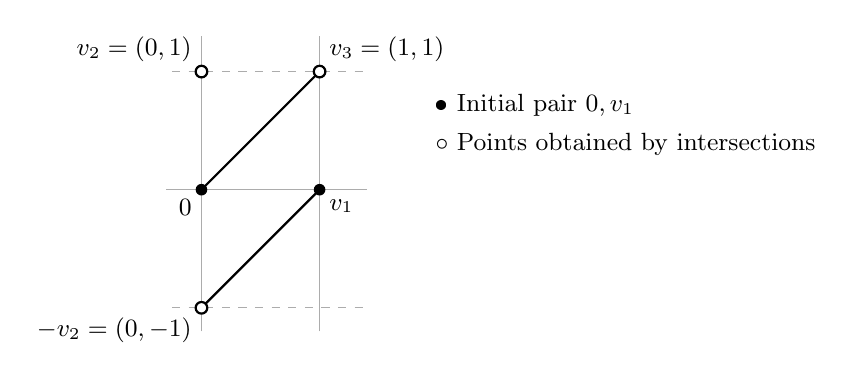
\begin{tikzpicture}[x=1.5cm,y=1.5cm,font=\small]
  \draw[gray!65] (-.3,0)--(1.4,0);
  \draw[gray!65] (0,-1.2)--(0,1.3);
  \draw[gray!65] (1,-1.2)--(1,1.3);
  \draw[gray!65,dashed] (-.25,1)--(1.4,1);
  \draw[gray!65,dashed] (-.25,-1)--(1.4,-1);
  \draw[thick] (0,0)--(1,1);
  \draw[thick] (0,-1)--(1,0);
  \fill (0,0) circle (2.1pt);
  \fill (1,0) circle (2.1pt);
  \draw[fill=white,thick] (1,1) circle (2.1pt);
  \draw[fill=white,thick] (0,1) circle (2.1pt);
  \draw[fill=white,thick] (0,-1) circle (2.1pt);
  \node[below left] at (0,0) {$0$};
  \node[below right] at (1,0) {$v_1$};
  \node[above right] at (1,1) {$v_3=(1,1)$};
  \node[above left] at (0,1) {$v_2=(0,1)$};
  \node[below left] at (0,-1) {$-v_2=(0,-1)$};
  \node[align=left,anchor=west] at (1.9,.55)
       {\textbullet\ Initial pair $0,v_1$\\[3pt]
        $\circ$\ Points obtained by intersections};
\end{tikzpicture}
\caption{The source-plane intersection construction using horizontal,
vertical and slope-one lines. The diagonal through $0$ meets the vertical
through $v_1$ at $v_3$; its horizontal gives $v_2$. The diagonal through
$v_1$ meets the vertical through $0$ at $-v_2$. Convergence of the image
intersections is proved in the text.}
\label{fig:three-foliation-grid}
\end{figure}

Fix $m\ge1$.  By the original two coordinate monotonicities,
$P F_j(v_1/m)$ is in the coordinate rectangle with vertices $0$ and
$P F_j(v_1)$, so it is bounded.  Every subsequential limit is $b v_1$
by the second hypothesis.  Apply the same finite intersection
construction with seed $v_1/m$ in place of $v_1$.  It constructs
$v_1$ after $m$ additions, and intersection convergence shows that
its limiting image is $mbv_1$.  Thus $mb=\sigma$.
This argument is valid even if one initially supposes $b=0$, since
every intersection is between two different line types.  Therefore
$F_j(v_1/m)\to\sigma v_1/m$ without a noncollapse assumption.
Repeating the grid construction proves convergence on
$(m^{-1}\mathbb Z)^2$, and hence at every rational point.

Finally squeeze each coordinate of $P F_j$ between the appropriate
corners of a rational grid cell.  The signs can differ between the
two coordinates and the two source axes; choose the lower and upper
corners for each coordinate separately.  The limiting corner values
are those of $\sigma P x$, whose oscillation on a cell is bounded by
a constant times its mesh.  A finite grid covering a compact set
therefore proves uniform convergence there.  This uses monotonicity
of $P F_j$, not an unjustified monotonicity of $F_j$.

For inverse convergence, choose a circle sufficiently large to contain
a given compact target set with positive margin.  Uniform convergence
on that circle and the Jordan curve theorem
(see \cite{Siebenmann2005}) show that its image
encloses the target set for large $j$; this image bounds the image of
the source disk.  The inverse images of the target set are thus
uniformly bounded.  Uniform convergence of $F_j$ on that disk gives
uniform convergence of the inverses.
\end{proof}

\subsection{Application to the rank coordinates}

Fix a rank point $p$ where all functions $f_C$ are differentiable and
where the directional conclusion already proved holds.  Choose three
times $\tau_1,\tau_2,\tau_3$ whose allowed direction sets are singletons
and are pairwise projectively distinct.  Let their unit directions
be $d_1,d_2,d_3$.  Fix an invertible matrix $B$ carrying
$[d_1],[d_2],[d_3]$ to $[v_1],[v_2],[v_3]$.

Consider any radii $h_j\downarrow0$ and indices tending sufficiently
fast that, on every bounded set of $w$ and for every fixed $C$,
\begin{equation}\label{eq:zoom-expansion}
 r_{C,j}(p+h_jw)=f_C(p)+h_j\nabla f_C(p)\cdot w+o(h_j).
\end{equation}
Here $r_{C,j}$ denotes the $C$ coordinate as a function of the pair
of rank coordinates, and the error is uniform on the bounded set.
This diagonal condition follows from monotone squeezing at continuity
points and differentiability at $p$.  It asserts no uniform rate in
the configuration index.

Normalize the original Euclidean plane linearly so its three
$\tau_i$ directions become $[v_i]$, translate the preimage of $p$ to
$0$, and scale the whole plane so the image of $v_1$ under the rank
zoom $B(r-p)/h_j$ has norm one.  Such a scale exists: on the chosen
horizontal ray the rank zoom is continuous, starts at zero, and exits
every fixed ball contained in its expanding target domain.
Let $F_j$ be this map from the normalized Euclidean plane to rank
zoom coordinates.

The first hypothesis of Lemma~\ref{lem:three-foliation} holds with
$P=B^{-1}$, by the two original rank-coordinate monotonicities;
passing to a subsequence fixes any orientation signs.  Its second
hypothesis follows from \eqref{eq:zoom-expansion}: every bounded limiting displacement on
a $\tau_i$ line satisfies all its directional sign constraints, so
it is parallel to $B d_i$, whether or not its base point moves.
The target domains exhaust the plane since $p$ is interior to the
rank square.  The lemma therefore applies.  In this normalization
the zoom and its inverse converge locally uniformly to a nonsingular
linear map; with the stated choice they converge to $\sigma I$.

We must compare this point-dependent normalization with the common
normalization based on three fixed times $t_1<t_2<t_3$: in each
configuration a linear map sends their projective directions to a
prescribed fixed triple.  Let $L_j$ map the open rank square to this
common normalized Euclidean plane, by inverting the rank map and
applying that linear map.  At our point
their allowed direction sets $D_p(t_i)$ are compact and pairwise
disjoint.  Let $\xi_{i,j}$ be their projective directions in the
$\tau$-normalized Euclidean plane.  After any further subsequence
these directions have limits.  Testing a unit segment through the
origin in direction $\xi_{i,j}$ in the uniformly convergent maps
shows that its limiting image direction, after undoing $B$, belongs
to the projectivization of $D_p(t_i)$.  Equivalently, orient the
tested segment in the original forward direction to obtain an
oriented limit in $D_p(t_i)$.  Thus the limiting directions lie in three fixed,
pairwise disjoint compact subsets of the projective line.  Their
separation is bounded below by a positive number depending only
on $p$ and the two fixed triples, independently of this zoom sequence.

Let $A_j$ convert the $\tau$ normalization to the common normalization,
which sends the $t_i$ directions to a prescribed fixed triple.
These matrices have bounded condition number.  Indeed normalize
$\|A_j\|=1$ and suppose a limit were singular.  At most one of three
separated limiting input directions could be its kernel, so two
others would have the same limiting output direction.  This
contradicts the two corresponding distinct fixed output directions.
Compactness gives a bound depending only on the separation and the
fixed target triple.

It follows that for every diagonal satisfying \eqref{eq:zoom-expansion}, after translations,
positive scalar rescalings and a subsequence, the common-coordinate
maps
\[
 w\longmapsto L_j(p+h_jw)-L_j(p)
\]
converge locally uniformly to an invertible linear map of condition
number at most $K_p<\infty$.  Indeed the normalized limit is
$\sigma A B$, with $A$ a nonsingular scalar-normalized limit of
$A_j$; the bound includes the fixed condition number of $B$.

Define
\[
 U_j(p,h)=\max_{|u-p|=h}|L_j(u)-L_j(p)|,
 \qquad
 V_j(p,h)=\min_{|u-p|=h}|L_j(u)-L_j(p)|.
\]
Choose $C_p>K_p$.  For each integer $T\ge2$, there exists
$h_{p,T}>0$ such that for every fixed $0<h<h_{p,T}$ and every
sufficiently late configuration $j$,
\begin{equation}\label{eq:radial-comparison}
 V_j(p,h/T)\ge\frac{U_j(p,h)}{C_p T},
 \qquad
 U_j(p,h/T)\le\frac{C_p V_j(p,h)}{T}.
\end{equation}
If either eventual comparison failed for arbitrarily small fixed
radii, choose radii tending to zero and failing indices arbitrarily
late, late enough also to satisfy \eqref{eq:zoom-expansion}.  Pass to the just-established
linear limit.  On the two circles its radial maxima and minima have
ratios $T\kappa$ and $\kappa/T$, respectively, with
$\kappa\le K_p<C_p$, contradicting failure.  This proves \eqref{eq:radial-comparison} in the
order stated: first the fixed radius, then the configuration index.

\section{A spatial measure with dimension greater than seven quarters}
\label{sec:spatial}

The boundary argument will count participating vertices, so it needs a
strip estimate for vertex mass while retaining a positive amount of edge
mass. We now construct a single Euclidean limit with these two properties.
The metric estimate from the preceding section concerns one fixed rank
point and radius at a time. A Hausdorff limit of graphs will allow us to
use it with configuration thresholds that still depend on the point
and radius.

Write $D=(0,1)^2$, and let $\pi:Z\to[0,1]^2$ be the projection onto the
rank coordinates $(z_A,z_B)$.  Denote the inverse rank maps, in the common
Euclidean normalization, by $L_n:D\to\mathbb R^2$.  These are
homeomorphisms.  For $\overline B(p,h)\subset D$, put
\[
 U_n(p,h)=\max_{|u-p|=h}|L_n(u)-L_n(p)|,
 \qquad
 V_n(p,h)=\min_{|u-p|=h}|L_n(u)-L_n(p)|.
\]
The input from the preceding section has the following exact quantifiers.
For each selected $p$, there is $C_p<\infty$ such that, for every integer
$T\ge2$, all sufficiently small fixed $h>0$ satisfy, eventually in $n$,
\begin{equation}
 V_n(p,h/T)\ge\frac{U_n(p,h)}{C_pT},
 \qquad
 U_n(p,h/T)\le\frac{C_pV_n(p,h)}{T}.
 \label{eq:spatial-metric-input}
\end{equation}
The constant $C_p$ is independent of $T$.  The allowed radii may depend on
$p,T$, and the eventual index may depend on $p,T,h$.

We use the positive good part already selected above: a Borel set
$E\subset Z$ with $\lambda_{K_0}(E)>0$, whose restricted endpoint measure
has absolutely continuous pair-coordinate projection, and for which
\eqref{eq:spatial-metric-input} holds at every $p\in\pi(E)$ after deleting
a null set.  We also retain $\lambda\ll\mu$.

The absolutely continuous projection here belongs to edge mass
$\lambda|_E$, not yet to the vertex mass $\mu|_E$ whose strip mass we
must bound. We will discard labels over a null set carrying the singular
part of the vertex projection and restrict its density to a bounded
range. The first deletion loses no selected edge mass, by absolute
continuity of its projection, and some finite density bound still
retains positive $\lambda_{K_0}$-mass. The metric construction will
then transfer this vertex-density bound from
rank coordinates to Euclidean disks and strips.

\begin{proposition}\label{prop:spatial-limit}
There is a Borel set $G\subset E$ with $\lambda_{K_0}(G)>0$, a further
subsequence, and a translation and uniform rescaling of each normalized
Euclidean plane with the following properties.  Over every
$p\in\pi(G)$ the limiting graph of the maps $L_n$ has a unique position
$l(p)$ in the closed unit disk.  With $\eta=1/16$, there is $c_G>0$ such
that
\begin{equation}
 |l(p)-l(q)|\ge c_G|p-q|^{1+\eta}
 \qquad(p,q\in\pi(G)).
 \label{eq:inverse-holder}
\end{equation}
Attach Euclidean position as an additional compactified coordinate to the
vertex measures, and take a weak limit $\widetilde\mu$.  Its restriction
by the old-label condition $z\in G$ has position marginal $\nu_G$
satisfying
\begin{equation}
 \nu_G(B(x,r))\le C_G r^{d_*},
 \qquad d_*=\frac{2}{1+\eta}=\frac{32}{17},
 \qquad x\in\mathbb R^2,\quad 0<r<1.
 \label{eq:disk-bound}
\end{equation}
Consequently every strip of width $r$ has $\nu_G$-mass at most
$C'_G r^{d_*-1}$, uniformly in its position and direction.  Every line
has zero $\nu_G$-mass.
\end{proposition}

\begin{proof}
We first select a positive set with common scale parameters and bounded
vertex density in the rank coordinates. After normalizing each
configuration at one common rank point, upper radial bounds will make the limiting graph single-valued
on that set, and lower radial bounds will give \eqref{eq:inverse-holder}.
Combining this estimate with the vertex density will prove the disk
and strip bounds.

For each integer $T\ge2$ and integer $m\ge0$, set
$h_j=T^{-m-j}$ and consider the points for which
$\overline B(p,h_0)\subset D$ and, for every $j\ge0$, eventually in $n$,
\begin{equation}
 \begin{aligned}
 V_n(p,h_{j+1})&\ge \alpha U_n(p,h_j),
 &\alpha&=T^{-1-\eta},\\
 U_n(p,h_{j+1})&\le \beta V_n(p,h_j),
 &\beta&=T^{-1+\eta}.
 \end{aligned}
 \label{eq:scale-radii}
\end{equation}
These are Borel conditions.  Indeed, at a fixed admissible radius,
$U_n$ and $V_n$ are continuous functions of the center, and eventual
validity is a countable union over starting indices followed by a
countable intersection over later indices.  Taking the further countable
intersection over $j$ preserves measurability.

For each point satisfying \eqref{eq:spatial-metric-input}, choose $T$
with $C_p\le T^\eta$, and then choose $m$ large enough.  This point
satisfies \eqref{eq:scale-radii} at all the selected radii.  The countable
union over $T,m$ therefore covers the selected good part.  Fix one pair
$T,m$ retaining positive $\lambda_{K_0}$-mass.  This selection makes no
claim of a common starting index.

The bounded density must concern vertices, since their activity will be
estimated later.  Decompose the pair-coordinate projection of the entire
vertex measure as
\[
 \pi_\#\mu=f(p)\,dp+\sigma_s,
 \qquad \sigma_s\perp dp.
\]
Choose an area-zero Borel carrier $S$ for $\sigma_s$, enlarged by any
area-zero set on which $f$ is not finite.  Delete $\pi^{-1}(S)$ from the
selected labels.  This loses no good mass because their endpoint
projection is absolutely continuous.  Next restrict to
$f(\pi(z))\le M$ for a sufficiently large finite $M$, retaining positive
$\lambda_{K_0}$-mass. Denote the resulting set by $G$; it satisfies
\begin{equation}
 \mu\bigl(G\cap\pi^{-1}(B)\bigr)\le M|B|
 \qquad\text{for every Borel }B\subset D.
 \label{eq:vertex-density}
\end{equation}
Here we have removed the singular part of the vertex projection and
truncated its density; absolute continuity of the endpoint projection
alone would not imply \eqref{eq:vertex-density}.

Cover $D$ by countably many balls of radius $h_0/8$ and restrict $G$ to
one of positive $\lambda_{K_0}$-mass.  Choose $p_0$ in its projected good
set.  Then
\[
 |p-p_0|<h_0/4\qquad(p\in\pi(G)).
\]
Translate and uniformly rescale the maps so that
\[
 L_n(p_0)=0,\qquad U_n(p_0,h_0)=1.
\]
The scale factor is positive, and \eqref{eq:scale-radii} is unchanged.

We next obtain bounds at every fixed scale, with constants independent of
the center.  For a homeomorphism, the image of a closed disk is a
topological closed disk whose boundary is the image of the boundary
circle.  Thus
\begin{equation}
 B(L_n(p),V_n(p,h))\subset L_n(B(p,h))
 \subset \overline B(L_n(p),U_n(p,h)).
 \label{eq:radial-enclosure}
\end{equation}
For the first inclusion, a segment from $L_n(p)$ to a missing point
closer than $V_n(p,h)$ would first leave the image through a closer
boundary point.  For the second, a positive maximum of the distance from
$L_n(p)$ cannot occur in the interior of the image disk.  Also, a point
outside $B(p,h)$ has image distance at least $V_n(p,h)$ from $L_n(p)$.

Since $T\ge2$, the localization gives
\[
 B(p_0,h_1)\subset B(p,h_0),
 \qquad
 \overline B(p,h_1)\subset B(p_0,h_0).
\]
Eventually $V_n(p_0,h_1)\ge\alpha$, so the first image contains $B(0,\alpha)$.
Its maximum distance from the possibly nonzero center $L_n(p)$ is at
least $\alpha$.  The second image is contained in the unit disk.  Therefore
\[
 U_n(p,h_0)\ge\alpha,\qquad U_n(p,h_1)\le2,
 \qquad |L_n(p)|\le1.
\]
Only the first inequality needs the anchor's eventual index.  The factor
$2$ occurs because $U_n(p,h_1)$ is measured from $L_n(p)$, rather than
from the origin.

Fix $p\in\pi(G)$ and an integer $j\ge1$.  Iterating the finitely many
inequalities \eqref{eq:scale-radii}, and using $V_n\le U_n$, gives,
eventually in $n$,
\begin{equation}
 V_n(p,h_j)\ge\alpha^{j+1},
 \qquad U_n(p,h_j)\le2\beta^{j-1}.
 \label{eq:iterated-radii}
\end{equation}
The constants are uniform over $G$.  The index threshold may depend on
$p,j$.  We will always fix these parameters before taking the limit.

The upper bounds in \eqref{eq:iterated-radii} tend to zero with the
scale, while the lower bounds keep distinct rank points separated.
We now pass to one graph limit in which both facts can be used, keeping
each center and scale fixed before taking the configuration limit.

To put all spatial limits on one subsequence, let $X$ be a compact metric
compactification of $\mathbb R^2$, and take the closures of the graphs
of $L_n$ in $[0,1]^2\times X$.  Pass to a subsequence on which these
compact sets converge in Hausdorff distance to a closed relation
$\Gamma$.  At an interior rank point, each finite-index closed graph
contains only the actual graph point, by continuity of $L_n$.

Fix $p\in\pi(G)$.  Its limiting fiber is nonempty by compactness,
because $|L_n(p)|\le1$.  Every $(p,x)\in\Gamma$ has graph-point
approximations $(u_n,L_n(u_n))$ at every sufficiently late index of the
same subsequence.  Since $u_n\to p$, eventually
$u_n\in B(p_0,h_0)$; consequently $|L_n(u_n)|\le1$.
Thus all points in this fiber have finite Euclidean positions.

Suppose $x$ and $y$ are two such positions.  Hausdorff convergence
provides approximations for both at the same indices.  Fix $j\ge1$.
Both rank arguments eventually lie in $B(p,h_j)$, where
\eqref{eq:radial-enclosure} and \eqref{eq:iterated-radii} bound the
distance between their positions by $4\beta^{j-1}$.  Passing to the limit
and then letting $j\to\infty$ proves $x=y$, since $\beta<1$.
Call this point $l(p)$.  Uniqueness also shows that $L_n(p)\to l(p)$
along the full selected subsequence.

For distinct $p,q\in\pi(G)$ put $d=|p-q|<h_0/2$.  Choose the first
$j\ge1$ with $h_j<d$; then $h_j\ge d/T$.  The point $q$ lies outside
the radius-$h_j$ disk centered at $p$, so eventually
\[
 |L_n(q)-L_n(p)|\ge V_n(p,h_j)\ge\alpha^{j+1}.
\]
Both fixed-point sequences converge on our subsequence.  Therefore
\[
 |l(q)-l(p)|\ge
 \alpha\left(\frac{h_j}{h_0}\right)^{1+\eta}
 \ge \frac{\alpha}{(Th_0)^{1+\eta}}\,d^{1+\eta},
\]
which proves \eqref{eq:inverse-holder}.  This argument uses a finite
number of scales for each fixed pair, not a common threshold over $G$.

Finally attach compactified position to the vertex and other spatial
measures before taking weak limits on this same subsequence.  Their
old-coordinate projections are unchanged.  Their pair-position
projections are supported on $\Gamma$: any compact set disjoint from
$\Gamma$ is disjoint from every sufficiently late closed graph, so
continuous tests supported there have limiting integral zero.
Consequently the enhanced vertex measure restricted by $z\in G$ lies
over the unique positions $l(\pi(z))$.  This restriction is made after
taking the limit; no convergence of finite-index restrictions to an
arbitrary Borel set $G$ is asserted.

If a disk of radius $r$ contains positions over $p$ and $q$, then
\eqref{eq:inverse-holder} gives
\[
 |p-q|\le (2r/c_G)^{1/(1+\eta)}.
\]
Thus its pair-coordinate preimage has planar outer area at most a
constant times $r^{2/(1+\eta)}$.  Applying
\eqref{eq:vertex-density} to that preimage proves
\eqref{eq:disk-bound}.  Using outer area avoids any requirement that a
projection of a Borel set itself be Borel.

The support of $\nu_G$ lies in the unit disk.  Its intersection with a
strip of width $r$ is covered by $O(1/r)$ disks of radius $O(r)$.
Summing \eqref{eq:disk-bound} proves the strip estimate; shrinking strips
to a line proves that lines have zero mass.
\end{proof}

The same enhancement preserves $\widetilde\mu_J\le\widetilde\mu$ and
all old marginals, in particular the positive mass
$\widetilde\lambda_{K_0}\{z\in G\}=\lambda_{K_0}(G)$.
By the enhanced-coordinate form of the earlier crossing inequality,
that inequality is also available on this selected set.  We will use the strip estimate
for its active-vertex measures.  The numerical fact needed below is
\[
 d_*=\frac{32}{17}>\frac74.
\]
This is an auxiliary spatial exponent; it is not the exponent saving in
the final halving-line bound.

\section{Boundary activity and the packing contradiction}
\label{sec:boundary}

We now use the spatial measure constructed above to rule out the assumed
sequence of extremal batches. The essential finite observation is that,
when the directions of the cutting lines vary little, every participating
vertex either lies in one of three narrow strips or is accounted for by
a marked token crossing the boundary of a fixed region. We first prove
this observation without taking limits.

\begin{lemma}[Three strips]
\label{lem:three-strips}
Let $P$ be a finite subset of $\mathbb R^2$, let $B$ be a bounded open set,
and let $D\geq1$ satisfy $|x|\leq D$ for $x\in B$. Suppose that
$M_0,\ldots,M_m\subset P$ have the same cardinality and are given by
strictly separating cuts
\[
 M_i=\{x\in P:\nu_i\cdot x<c_i\},
 \qquad |\nu_i|=1,
 \qquad |\nu_i-\nu_0|\leq\theta.
\]
For each $i\geq1$, choose a bijection from $M_{i-1}\setminus M_i$ to
$M_i\setminus M_{i-1}$. Let $C_B$ count the resulting transfers having
exactly one endpoint in $B$, and let
\[
 A=\bigcup_{i=1}^m(M_{i-1}\mathbin\triangle M_i)
\]
be the set of distinct participating vertices. Set
\[
 \rho=D\theta,\qquad c_- =\min_{0\leq i\leq m}c_i,
 \qquad c_+=\max_{0\leq i\leq m}c_i,
\]
and, for $q\in\{c_0,c_-,c_+\}$, define the closed strip
\[
 S_q=\{x\in\mathbb R^2:|\nu_0\cdot x-q|\leq3\rho\}.
\]
Then
\[
 \#\bigl((A\cap B)\setminus(S_{c_0}\cup S_{c_-}\cup S_{c_+})\bigr)
 \leq2C_B,
\]
and consequently
\begin{equation}
 \#(A\cap B)
 \leq 2C_B+
 \sum_{q\in\{c_0,c_-,c_+\}}\#(P\cap B\cap S_q).
 \label{eq:finite-three-strips}
\end{equation}
Repeated thresholds may be counted repeatedly in the sum.
\end{lemma}

\begin{proof}
Write $t(x)=\nu_0\cdot x$ and
$e_i(x)=(\nu_i-\nu_0)\cdot x$. For $x\in B$ we have
$|e_i(x)|\leq\rho$, and $e_0(x)=0$. Put
$S=S_{c_0}\cup S_{c_-}\cup S_{c_+}$.
Figure~\ref{fig:three-strip-projection} shows the two ranges in which
participants in $B$ outside $S$ can occur. We compare their membership with
the states attaining the minimum and maximum thresholds.

\begin{figure}[htbp]
\centering
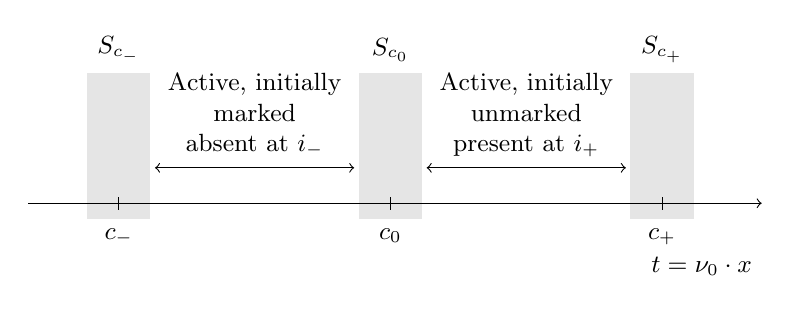
\begin{tikzpicture}[x=1.15cm,y=1cm,font=\small]
  \fill[gray!20] (.65,-.2) rectangle (1.35,1.65);
  \fill[gray!20] (3.65,-.2) rectangle (4.35,1.65);
  \fill[gray!20] (6.65,-.2) rectangle (7.35,1.65);
  \draw[->] (0,0)--(8.1,0);
  \draw (1,-.08)--(1,.08);
  \draw (4,-.08)--(4,.08);
  \draw (7,-.08)--(7,.08);
  \node[below] at (1,-.2) {$c_-$};
  \node[below] at (4,-.2) {$c_0$};
  \node[below] at (7,-.2) {$c_+$};
  \node[anchor=east] at (8.1,-.8) {$t=\nu_0\cdot x$};
  \node at (1,1.95) {$S_{c_-}$};
  \node at (4,1.95) {$S_{c_0}$};
  \node at (7,1.95) {$S_{c_+}$};
  \draw[<->] (1.4,.45)--(3.6,.45);
  \draw[<->] (4.4,.45)--(6.6,.45);
  \node[align=center] at (2.5,1.12)
    {Active, initially\\marked\\absent at $i_-$};
  \node[align=center] at (5.5,1.12)
    {Active, initially\\unmarked\\present at $i_+$};
\end{tikzpicture}
\caption{Projection onto $t=\nu_0\cdot x$. The shaded bands have
half-width $3\rho$; their separation is schematic, and in general they
may overlap. An initially marked participant in $B$ outside the bands is lost
by a state $i_-$ attaining $c_-$; this endpoint comparison has no gains
inside $B$.
The symmetric statement holds for initially unmarked participants and
a state $i_+$ attaining $c_+$. Token conservation bounds these two
numbers by exits and entries, respectively. This is an aggregate count;
it does not assign each participant's own token to a boundary crossing.}
\label{fig:three-strip-projection}
\end{figure}

Consider first an $x\in(A\cap B)\setminus S$ that is initially marked.
Avoidance of $S_{c_0}$ gives $t(x)<c_0-3\rho$. Since $x$ participates,
it is unmarked at some boundary state, and hence
$t(x)+e_i(x)>c_i\geq c_-$ at some $i$. Therefore
$t(x)>c_- -\rho$. Avoidance of $S_{c_-}$ improves this to
$t(x)>c_-+3\rho$. At an index $i_-$ attaining the minimum threshold,
\[
 \nu_{i_-}\cdot x\geq t(x)-\rho>c_-;
\]
thus $x$ is lost between states $0$ and $i_-$. The existence of even one
such $x$ also forces $c_0-c_->6\rho$. Consequently every initially
unmarked $y\in P\cap B$ is still unmarked at state $i_-$, because
\[
 \nu_{i_-}\cdot y\geq t(y)-\rho>c_0-\rho>c_-.
\]
There are therefore no gains anywhere inside $B$ in this comparison,
including among vertices lying in the strips.

To count the losses, place one distinct token on each point of $M_0$.
At every step retain the tokens on unchanged marked vertices and move
the others along the chosen matching. There is exactly one token on
every marked vertex at each state. It follows that
\[
 \#(M_0\cap B)-\#(M_{i_-}\cap B)
 =\text{token exits from }B-\text{token entries into }B
\]
over that prefix of steps. Since all differences between these two states inside $B$ are losses,
their number equals this difference and is at most $C_B$. This bounds
the initially marked participants outside the strips; if there are
none, the bound holds without imposing a threshold gap.

Now let $x\in(A\cap B)\setminus S$ be initially unmarked. It satisfies
$t(x)>c_0+3\rho$ and is marked at some later state, so
$t(x)<c_++\rho$. Avoidance of $S_{c_+}$ implies
$t(x)<c_+-3\rho$. At an index $i_+$ attaining $c_+$,
\[
 \nu_{i_+}\cdot x\leq t(x)+\rho<c_+,
\]
so $x$ is gained by that state. If this class is nonempty, then
$c_+-c_0>6\rho$. Every initially marked $y\in P\cap B$ consequently
remains marked at state $i_+$, since
\[
 \nu_{i_+}\cdot y\leq t(y)+\rho<c_0+\rho<c_+.
\]
All differences between these two states inside $B$ are gains, and token
conservation bounds their number by $C_B$. The two classes together
contain at most $2C_B$ vertices, proving
\eqref{eq:finite-three-strips}.

The argument includes $\theta=0$, when the strips are lines. It also
includes vertices that change membership several times and return to
their initial status: participation requires only that some boundary
state differs from the initial one.
\end{proof}

We apply this lemma only to states separating consecutive batches.
Thus its set $A$ is exactly the set of endpoints participating in the
batch exchange graph. A membership change within a batch followed by
a return before its end does not by itself contribute a vertex to $A$
or to the measure $\mu_J$; that vertex may still participate at another
batch boundary.

For the rest of this section, suppress the tildes on the enhanced
measures from Section~\ref{sec:spatial}, and write $\widetilde Z$ for
their compact label space, which includes compactified Euclidean position. The
condition $z\in G$ always refers to the old rank label, pulled back to
$\widetilde Z$. Thus expressions such as $\mu_J(G)$ refer to the
enhanced measures restricted by that condition.

Recall the particular inputs furnished by the preceding construction.
There is a dyadic window $K_0$, a measurable label set $G$, and limiting
measures with
\begin{equation}
 \begin{gathered}
 \lambda_{K_0}(G)>0,\qquad \mu_J\leq\mu,\qquad
 \lambda_J(\widetilde Z)=|J|,\\
 \lambda_J(F)^3\leq C s_J^3\mu_J(F).
 \end{gathered}
 \label{eq:boundary-measure-input}
\end{equation}
for every Borel set $F\subset\widetilde Z$ and every dyadic $J\subset K_0$.
Here $s_J$ is the limiting fraction of distinct participating batch
endpoints. At every dyadic resolution $\delta$,
\begin{equation}
 \#\{J\subset K_0:|J|=\delta,\ s_J>u\}
 \leq C u^{-4/3}.
 \label{eq:boundary-packing-input}
\end{equation}
The spatial projection $\beta$ of $\mu|_G$ is boundedly supported and
satisfies
\begin{equation}
 \beta(B(x,r))\leq C_G r^d,
 \qquad 0<r<1,
 \qquad d=\frac{32}{17}>\frac74.
 \label{eq:boundary-disk-input}
\end{equation}
These masses are unchanged because the enhancement preserved all the
original measure projections.

The directions throughout $K_0$ lie between the directions at its two
fixed bracketing times. The common linear normalization sends those
two projective directions to distinct fixed directions. Passing to a
subsequence selects one of the two projective arcs between them and
one of its two oriented lifts. Hence all forward transfer vectors lie
in a fixed closed cone $\mathcal C$ of aperture less than $\pi$.
We may enlarge this cone slightly and discard finitely many indices. Each intermediate
forward transfer vector is a positive linear combination of the two
bracketing forward vectors; this identifies the relevant cone after
normalization, including its orientation.

Choose linearly independent covectors $\ell_1,\ell_2$ in the interior
of its dual cone. Thus $\ell_j(v)>0$ for every nonzero
$v\in\mathcal C$. Choose a bounded open parallelogram
\[
 B=\{x:a_1<\ell_1(x)<b_1,\ a_2<\ell_2(x)<b_2\}
\]
whose interior contains the support of $\beta$, and fix
$D\geq\max(1,\sup_{x\in B}|x|)$.

For every batch choose one perfect matching between its $a$ lost and
$a$ gained marked vertices, making this choice once throughout $K_0$.
Follow the resulting system of at most $N$ marked tokens. Each side
functional is monotone along every token trajectory, so each token
crosses each of the four side levels of $B$ at most once. Therefore
there are at most $4N$ matching transfers with one endpoint inside $B$
and one outside during the entire window $K_0$.

Let $C_n(J)$ be the number of these transfers during $J$ in
configuration $n$. Let $\theta_n(J)$ be the angular width of the span
of its boundary-state directions in the normalized plane. These
directions rotate monotonically, and the spans of disjoint windows
have disjoint interiors. Thus, for every dyadic partition of $K_0$,
\[
 \sum_J \frac{C_n(J)}{N_n}\leq4,
 \qquad \sum_J\theta_n(J)\leq\pi.
\]
A diagonal subsequence on the countable family of windows gives
limits $b_J$ and $\theta_J$ with
\begin{equation}
 \sum_J b_J\leq4,\qquad \sum_J\theta_J\leq\pi.
 \label{eq:boundary-budgets}
\end{equation}
These are limits at a fixed time resolution; no assertion of uniform
convergence over resolutions is needed.

\begin{lemma}[Limiting boundary activity]
\label{lem:limiting-boundary-activity}
For each dyadic $J\subset K_0$,
\begin{equation}
 \mu_J(G)\leq2b_J+C_G\theta_J^{d-1}.
 \label{eq:limiting-boundary-activity}
\end{equation}
\end{lemma}

\begin{proof}
Apply Lemma~\ref{lem:three-strips} to the finite boundary states of
$J$. Continuously orient their unit normals so that the marked sets
are given by $\nu_i\cdot x<c_i$. Their angular span is
$\theta_n(J)$, and consequently $|\nu_i-\nu_0|\leq\theta_n(J)$.

Pass further to a subsequence so that the initial normal and the
initial, minimum and maximum thresholds converge, allowing infinite
threshold limits. This can be done simultaneously for the countably
many windows. A finite threshold limit gives a limiting closed strip
of half-width $3D\theta_J$. A threshold tending to either infinity
gives strips that eventually miss every bounded set. Let $\mathcal S_J$ be
the union of the nonescaping limiting strips.

Let $\alpha_n$ be the spatial projection of the participating-vertex
measure in $J$, normalized by $N_n$, and let $\alpha$ be its weak
limit. Any continuous function $f$ with $0\leq f\leq1$ and compact
support in $B\setminus\mathcal S_J$ eventually avoids all three moving strips.
Lemma~\ref{lem:three-strips} therefore gives
\[
 \int f\,d\alpha_n\leq 2C_n(J)/N_n.
\]
Passing to the limit and exhausting the open set by such tests yields
$\alpha(B\setminus\mathcal S_J)\leq2b_J$. Since the positions carrying
$\mu|_G$ lie inside $B$, and $\mu_J\leq\mu$, it follows that
\[
 \mu_J(G)\leq2b_J+\beta(\mathcal S_J).
\]
This argument restricts to $G$ only after weak convergence; no
convergence of finite restrictions to $G$ has been assumed.

To bound the remaining term, cover the intersection of a strip of
half-width $r$ with the bounded support of $\beta$ by $O_G(r^{-1})$
disks of radius $O(r)$. Equation~\eqref{eq:boundary-disk-input} gives
\[
 \beta(\text{strip of half-width }r)\leq C_G r^{d-1}
 \qquad(0<r<1).
\]
For larger widths the same estimate follows from the total mass bound
after increasing $C_G$. A line has zero $\beta$-mass by continuity
from above, since $d>1$. Applying this bound to the at most three
limiting strips proves the result, including $\theta_J=0$.
\end{proof}

It remains to combine this activity bound with the endpoint estimate.
Fix $M\geq1$ and subdivide $K_0$ into dyadic windows of length
$\delta$. By \eqref{eq:boundary-packing-input}, the number with
$s_J>M\delta^{3/4}$ is at most
$C M^{-4/3}\delta^{-1}$. Each has total $\lambda_J$-mass $\delta$,
so these windows contribute at most $C M^{-4/3}$ to
$\lambda_{K_0}(G)$.

For the other windows, \eqref{eq:boundary-measure-input} gives
\[
 \sum_{s_J\leq M\delta^{3/4}}\lambda_J(G)
 \leq C M\delta^{3/4}\sum_J\mu_J(G)^{1/3}.
\]
There are at most $\delta^{-1}$ windows. Set
$\alpha=d-1=15/17\in(0,1)$. H\"older's inequality,
Lemma~\ref{lem:limiting-boundary-activity}, and
\eqref{eq:boundary-budgets} imply
\[
 \sum_J\mu_J(G)^{1/3}
 \leq \delta^{-2/3}\Bigl(\sum_J\mu_J(G)\Bigr)^{1/3}
 \leq C_G\delta^{-2/3}
       \Bigl(1+\sum_J\theta_J^\alpha\Bigr)^{1/3}.
\]
Concavity and the angular budget give
\[
 \sum_J\theta_J^\alpha
 \leq \delta^{\alpha-1}\Bigl(\sum_J\theta_J\Bigr)^\alpha
 \leq C\delta^{\alpha-1}.
\]
Consequently
\begin{align*}
 \lambda_{K_0}(G)
 &\leq C M^{-4/3}
      +C_G M\delta^{-1/4}(\delta+\delta^{d-1})^{1/3}\\
 &\leq C M^{-4/3}
      +C_G M\bigl(\delta^{1/12}+\delta^{3/68}\bigr),
\end{align*}
where
\[
 \frac{d-1}{3}-\frac14
 =\frac{15}{51}-\frac14=\frac{3}{68}>0.
\]
First let $\delta\downarrow0$ with $M$ fixed, and then let
$M\to\infty$. This contradicts $\lambda_{K_0}(G)>0$ and excludes
the proposed sequence of extremal batches. Together with the finite
reductions, it establishes the uniform little-$o$ activity-packing
estimate. The numerical exponent $3/68$ concerns only this limiting
contradiction; the power saving in the final finite theorem is chosen
separately.

\section{From activity packing to a power saving}
\label{sec:recurrence}

We now turn the uniform activity-packing estimate into a fixed power
improvement. The scale is chosen once and then used at every size in
an induction. Throughout this section, a sweep is the ordering by
increasing values of $y-sx$ as $s$ runs from $-\infty$ to $+\infty$.
Its rank-$k$ marked set consists of the $k$ smallest values. The
\emph{activity} of an interval of sweep steps is the number of distinct
points whose membership in that set changes during the interval.

\begin{proposition}\label{prop:packing-to-power}
Suppose that, for every $\eta>0$, there is $R_\eta<\infty$ such that
for every generic planar configuration of $N$ points, every rank, and
every integer $1\le b\le N$ with $N/b\ge R_\eta$, the number of
step-disjoint intervals of activity at least $b$ is at most
$\eta(N/b)^{4/3}$. Then there are absolute constants $\varepsilon>0$
and $C$ such that every such rank sweep has at most
$CN^{4/3-\varepsilon}$ switches.
\end{proposition}

\begin{proof}
Write $a=4/3$, set $\eta=(4\cdot2^a)^{-1}$, and choose an integer
$q\ge\max\{4,R_\eta\}$. This integer remains fixed. For $N\ge4q$,
put
\[
 d=\lfloor N/q\rfloor,\qquad b=d-1.
\]
Then $N/(2q)\le b<N/q$, so the packing hypothesis applies and
$N/b\le2q$.

Partition the sweep greedily, ending a block when its activity first
reaches $b$, and include any final remainder. Immediately before the
last step of a completed block, the activity is at most $b-1$.
A step changes at most two memberships, so the block has at most
$b+1=d$ active points. The remainder has fewer than $b$ active points.
The completed blocks are step-disjoint, and hence their number is at
most
\[
 \eta(N/b)^a\le\eta(2q)^a=q^a/4.
\]
Including the one possible remainder gives at most $q^a/2$ blocks,
since $q^a\ge4$. Every block uses at most $N/q$ active points.

Let $A$ be the active points of one block and let $B$ be the points
outside $A$ that are marked at its initial state. Membership of every
point outside $A$ is constant during the block. Therefore restriction
to $A$ is a sweep at the fixed rank $r=k-|B|$: at every state, the
marked points of $A$ are exactly its $r$ lowest points. This identity
also proves that the switches in the block are exactly the switches
of the restricted rank-$r$ sweep over that slope interval. Their
number is bounded by the complete-sweep complexity on $|A|$ points.

Let $F(n)$ be the largest switch count among all generic configurations
of exactly $n$ points and all ranks, with $F(0)=F(1)=0$. It is finite,
since $F(n)\le\binom n2$. Set
\[
 \varepsilon=\frac{\log2}{2\log q},\qquad
 \beta=\frac43-\varepsilon>0.
\]
Choose $C$ so that $F(n)\le Cn^\beta$ for $1\le n<4q$. Suppose this
bound holds at every size smaller than $N\ge4q$. If $t_j\le N/q$
are the active-subset sizes of the blocks, the restriction argument
and the induction hypothesis give
\[
 F(N)\le\sum_j F(t_j)
 \le C\sum_j t_j^\beta
 \le C\frac{q^a}{2}\left(\frac Nq\right)^\beta
 =\frac{C}{\sqrt2}N^\beta
 \le CN^\beta.
\]
Here every nonempty subset has size less than $N$, while empty subsets
contribute zero. Thus induction proves the assertion for all sizes
and ranks. The selection of $q$ from $R_\eta$ is nonquantitative;
this argument does not provide a numerical value of $\varepsilon$.
\end{proof}

Proposition~\ref{prop:packing-to-power} and Theorem~\ref{thm:activity-packing}
prove Theorem~\ref{thm:all-ranks}. It remains to transfer its middle-rank
case to the configurations of Theorem~\ref{thm:halving-power}.

For a generic configuration of $N=2m$ points, a pair is halving
precisely when its critical slope ties positions $m$ and $m+1$:
there are then $m-1$ points on each side of its line. The two tied
points exchange order, so halving pairs are exactly the middle-rank
switches. Each unordered pair has one critical slope in this sweep.
The perturbation argument in Section~\ref{sec:finite} preserves all
halving pairs of an arbitrary configuration with no three collinear. Consequently
Proposition~\ref{prop:packing-to-power}, applied to Theorem~\ref{thm:activity-packing}, gives the asserted bound for every even
size and every such configuration.

\subsection{Planar \texorpdfstring{$k$}{k}-sets and straight-line levels}
\label{sec:k-sensitive-proof}

We finish by deriving the rank-sensitive consequence stated in the
introduction. The local ranks created by a shallow cutting can vary from
cell to cell, which is why the uniform sweep theorem was needed.

\begin{proof}[Proof of Corollary~\ref{cor:k-sensitive}]
Take $\varepsilon$ from Theorem~\ref{thm:all-ranks} and set
$\varepsilon_0=\min\{\varepsilon,1/6\}$ and
$\beta=4/3-\varepsilon_0>1$. The theorem remains valid with exponent
$\beta$ in place of $4/3-\varepsilon$.

Dualize a point $(a,b)$ to the line $y=b-as$. For a generic dual point
set $P$, let $V_j$ be the arrangement vertices with exactly $j$ lines
strictly below them. Then $|V_j|=S_{j+1}(P)$: at such a vertex the lines
in positions $j+1$ and $j+2$ exchange order. The vertices of
$\Lambda_j$ are $V_{j-1}\cup V_j$, with out-of-range sets empty
\cite[Section~1, p.~2]{AgarwalAronovChanSharir1998}. Thus
Theorem~\ref{thm:all-ranks} bounds every level of $M$ dual lines by
$O(M^\beta)$ vertices, uniformly in its rank; its number of edge pieces
is one more than its number of vertices. For any line arrangement in
the corollary, the dual point set has no three collinear and distinct
first coordinates. The perturbation in Section~\ref{sec:finite} can
also preserve the order of those coordinates, so its preservation of
all triple-orientation signs preserves every dual vertex's number of
lines below it. The uniform $O(M^\beta)$ level bound therefore holds
for every such general-position line arrangement.

Apply Matou\v{s}ek's shallow-cutting lemma in the form stated by
Agarwal, Aronov, Chan, and Sharir
\cite[Lemma~3.2 and the following reduction, pp.~10--11]{AgarwalAronovChanSharir1998}.
In dimension two, take $r=n/(k+1)\ge1$ and
$q=kr/n+1<2$. The cutting has $O(rq)=O(n/(k+1))$ cells, each crossed
by at most $n/r=k+1$ lines. Within the interior of a cell, the
noncrossing lines give a fixed rank offset, so the part of the global
level has one fixed local rank in the arrangement of crossing lines.
This local rank need not
equal $k$, which is why the all-ranks bound is used. Boundary pieces
cost $O(k+1)$ per cell: each crossing line meets the simplex boundary
at most twice. An input line not crossing the interior can contribute
only along a side or at a vertex. General position allows at most one
such line per side and at most two through each vertex; the already
counted intersections split their contributions into $O(k+1)$ pieces
in total. Since $\beta>1$, these terms are absorbed by the local
$O((k+1)^\beta)$ bound. The cited shallow-cutting reduction now gives
\[
 \operatorname{comp}\bigl(\Lambda_k(\mathcal L)\bigr)
 =O\bigl(r(n/r)^\beta\bigr)
 =O\bigl(n(k+1)^{1/3-\varepsilon_0}\bigr).
\]

For a generic point set $Q$, every $k$-set consists of the $k$ smallest
values of some linear functional. Normal directions with positive
second coordinate give the bottom-$k$ sweep, while those with negative
second coordinate give complements of the bottom-$(n-k)$ sweep.
The horizontal directions are included by limits, since first
coordinates are distinct. Hence the number of $k$-sets is at most
$S_k(Q)+S_{n-k}(Q)+2$. In the dual arrangement,
$S_k(Q)=|V_{k-1}|$; vertical reflection sends the vertices counted by
$S_{n-k}(Q)=|V_{n-k-1}|$ to $V_{k-1}$ of the reflected arrangement.
Each of these two vertex sets
lies on a $k$-th level, so the level bound just proved applies twice.
Finally, for any fixed point set, choose one strict separating line for
each of its finitely many $k$-sets. All these strict separations survive
a sufficiently small generic perturbation. Its original number of
$k$-sets is therefore no larger than the generic count.
\end{proof}

\begingroup
\raggedright
\bibliographystyle{plainnat}
\bibliography{references}
\endgroup
\end{document}
